\chapter{Lab 03 --- Customer Segmentation}
\label{ch:lab03}

\section{Problem Definition}

\begin{problembox}
Group mall customers into interpretable, actionable segments using \textbf{unsupervised clustering}. The goal is not to optimize a single metric, but to produce groups with clear behavioral signatures that a marketing team can immediately act upon. Success criteria: \textbf{silhouette score $> 0.300$}, clusters \textbf{$> 5\%$ of total customers}, and semantically meaningful labels (e.g., ``High Income, High Spending'').
\end{problembox}

\subsection{Dataset}
\begin{itemize}
  \item \textbf{Source:} Shopping Mall Customer Segmentation Data (Kaggle), 2,200 rows, shape $(2200, 5)$.
  \item \textbf{Features:} \texttt{Age} (18--90), \texttt{Annual Income} (k\$), \texttt{Spending Score} (1--100), \texttt{Gender} (optional one-hot), \texttt{CustomerID} (excluded --- it is a label, not a measurement).
  \item \textbf{Data quality:} 0 missing values, 0 duplicate rows --- clean dataset requiring no imputation or deduplication before modeling.
\end{itemize}

\section{Complete Workflow}

\subsection{Reproducibility Setup}
A fixed random seed (42) ensures centroid initialization is deterministic across runs. Four local modules (\texttt{utils}, \texttt{preprocess}, \texttt{eda}, \texttt{clustering}) encapsulate logic; \texttt{importlib.reload()} enables code edits without kernel restart. All figures and preprocessing reports are saved to versioned directories so that each experiment leaves an auditable artifact trail.

\subsection{Raw Data Overview}
\texttt{utils.find\_raw\_csv()} discovers the dataset via a configurable glob pattern --- no hardcoded filename. Column names are normalized to \texttt{customer\_id}, \texttt{gender}, \texttt{age}, \texttt{annual\_income}, \texttt{spending\_score} for consistent downstream access. The printed overview (shape, dtypes, missing, duplicates, descriptive statistics) serves as the first quality gate: any unexpected dtype or out-of-range value is caught here before it propagates into later pipeline stages.

\subsection{Data Quality Checks}
Four issues are catalogued before any transformation:
\begin{itemize}
  \item \textbf{Missing values:} Per-column count and percentage. The dataset has 0 missing values across all columns.
  \item \textbf{Duplicates:} Exact row comparison. The dataset has 0 duplicate rows; had duplicates exceeded 1\% of total rows, investigation into data collection errors would be required.
  \item \textbf{Invalid ranges:} Age 0--120, income $\ge$ 0, spending 1--100. Negative income or ages above 150 would signal data corruption.
  \item \textbf{Outliers:} Both z-score ($|z| > 3$) and IQR ($Q1-1.5\times\text{IQR}$ to $Q3+1.5\times\text{IQR}$) methods. Outliers are summarized, \textbf{not removed} --- the report quantifies deviations for informed case-by-case decisions. The IQR method flags more points for right-skewed income data because it does not assume symmetry, making it more sensitive to the long upper tail of the income distribution.
\end{itemize}

A preprocessing report (markdown) is saved for audit trail, recording every detected anomaly alongside its column, row index, and deviation magnitude.

\begin{figure}[H]
  \centering
  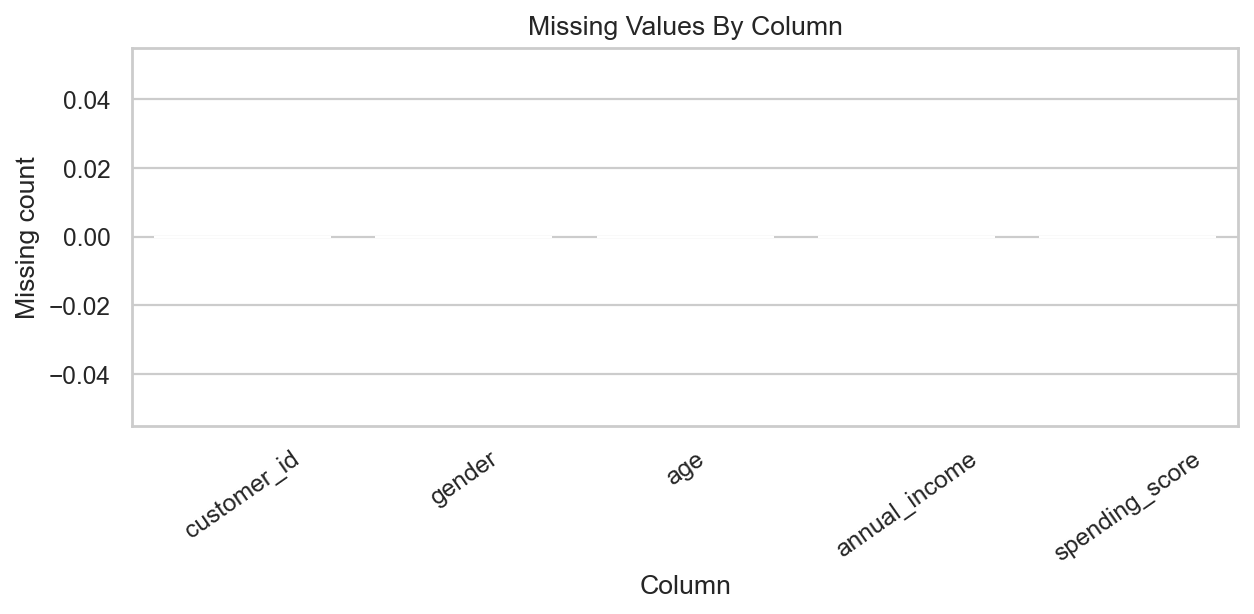
\includegraphics[width=\textwidth]{figures/lab03/missing_values.png}
  \caption{Missing values per column --- all columns show 0.000\% missing, confirming no imputation is needed.}
\end{figure}

\begin{figure}[H]
  \centering
  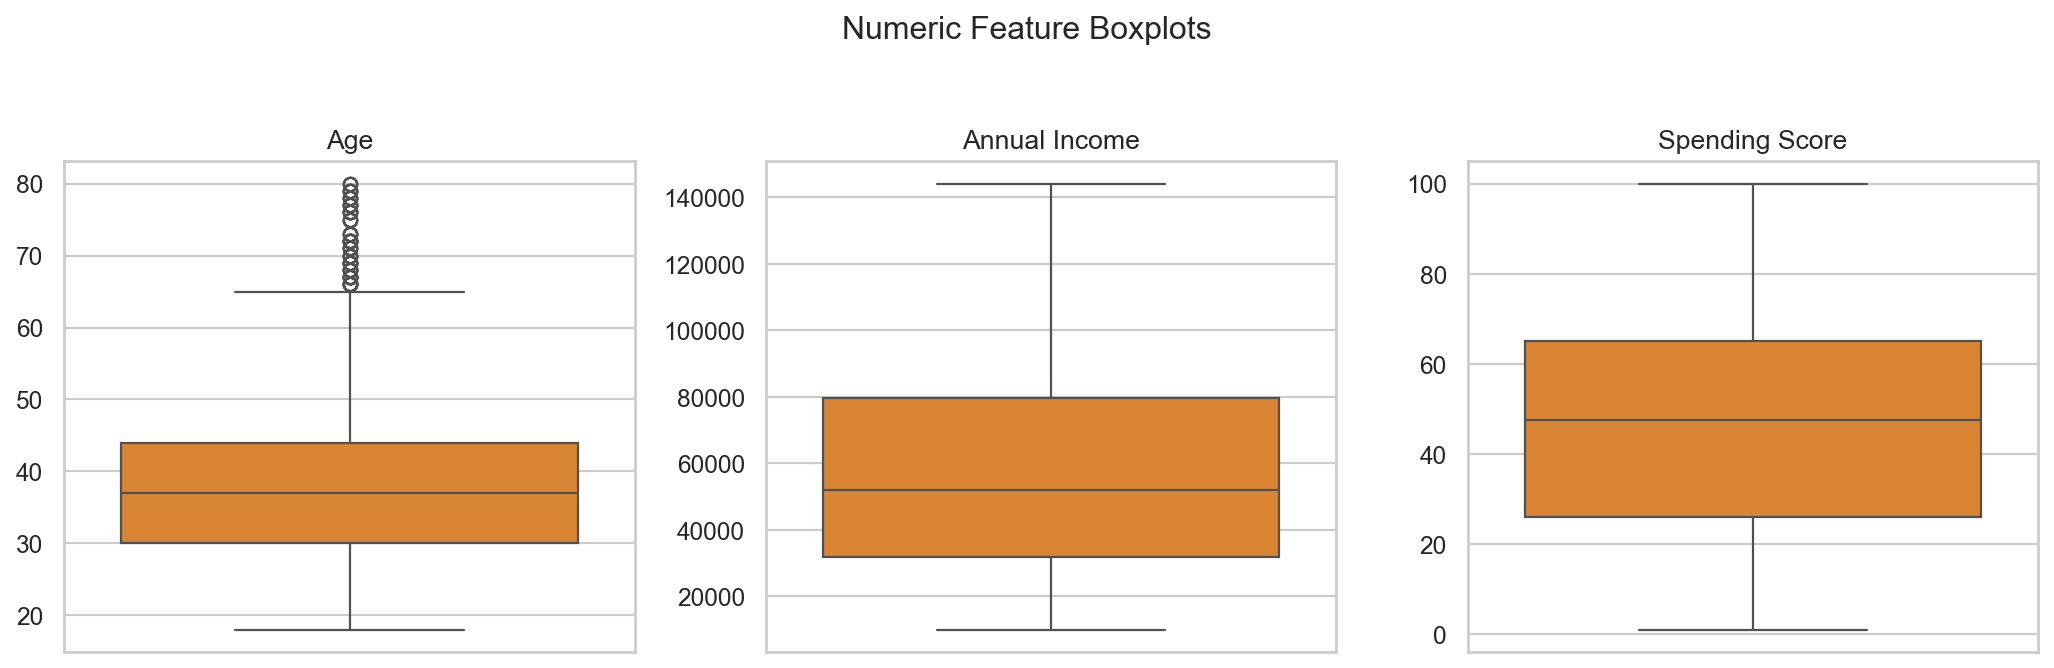
\includegraphics[width=\textwidth]{figures/lab03/boxplots_before.png}
  \caption{Boxplots on original scale --- income exhibits a right-skewed distribution with a long upper tail; age and spending score are more symmetric.}
\end{figure}

\begin{figure}[H]
  \centering
  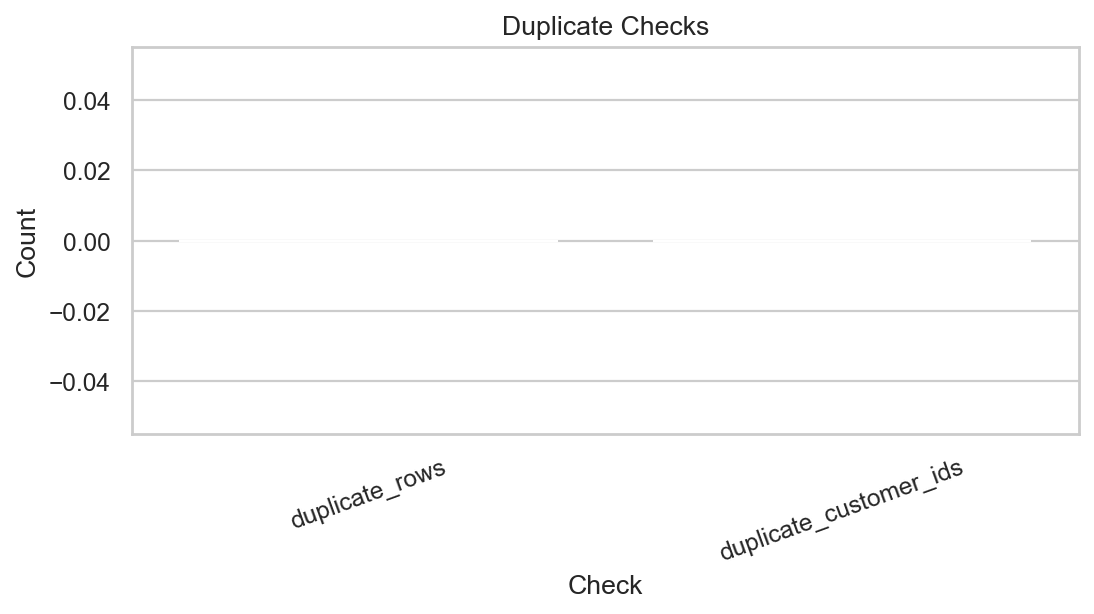
\includegraphics[width=0.700\textwidth]{figures/lab03/duplicate_summary.png}
  \caption{Duplicate row summary --- 0 exact row matches detected, confirming the $(2200, 5)$ dataset has no redundant observations.}
\end{figure}

\subsection{EDA Before Preprocessing}

EDA runs in \textbf{original units} --- before scaling abstracts the numbers away. Six plots cover the full picture:

\begin{table}[H]
\centering\rowcolors{2}{tablerow}{white}
\begin{tabular}{l L{8cm}}
\toprule\rowcolor{tablehead!80}\color{white}\textbf{Plot} &\color{white}\textbf{Key Question}\\
\midrule
Histograms/KDE & Are age, income, spending uniformly distributed? Bimodal spending suggests natural clusters.\\
Gender distribution & Is the customer base balanced? A skew $> 70/30$ should be noted.\\
Income vs.\ Spending scatter & \textbf{Most important plot.} Do 4--6 visually separable clouds appear? If yes, clustering will succeed.\\
Age vs.\ Spending scatter & Does age predict spending? A downward trend is actionable for age-targeted campaigns.\\
Age vs.\ Income scatter & Are older customers wealthier?\\
Correlation heatmap & Any $|r| > 0.700$ indicates redundant features that can be dropped.\\
Pairplot & All pairwise scatters in one grid --- catches interactions a correlation coefficient would miss.\\
\bottomrule
\end{tabular}
\caption{EDA before preprocessing --- 6 diagnostic views}
\end{table}

The \textbf{Income vs.\ Spending scatter} is the most important plot in the entire notebook. The classic Mall Customers dataset typically shows \textbf{5 distinct clusters}: high/high, high/low, medium/medium, low/high, low/low. Each cluster represents a coherent spending-income behavioral profile that maps directly to a marketing strategy. The visual separation between these clusters is sufficient that even simple K-Means reliably recovers them without requiring kernel methods or spectral clustering.

\begin{figure}[H]
  \centering
  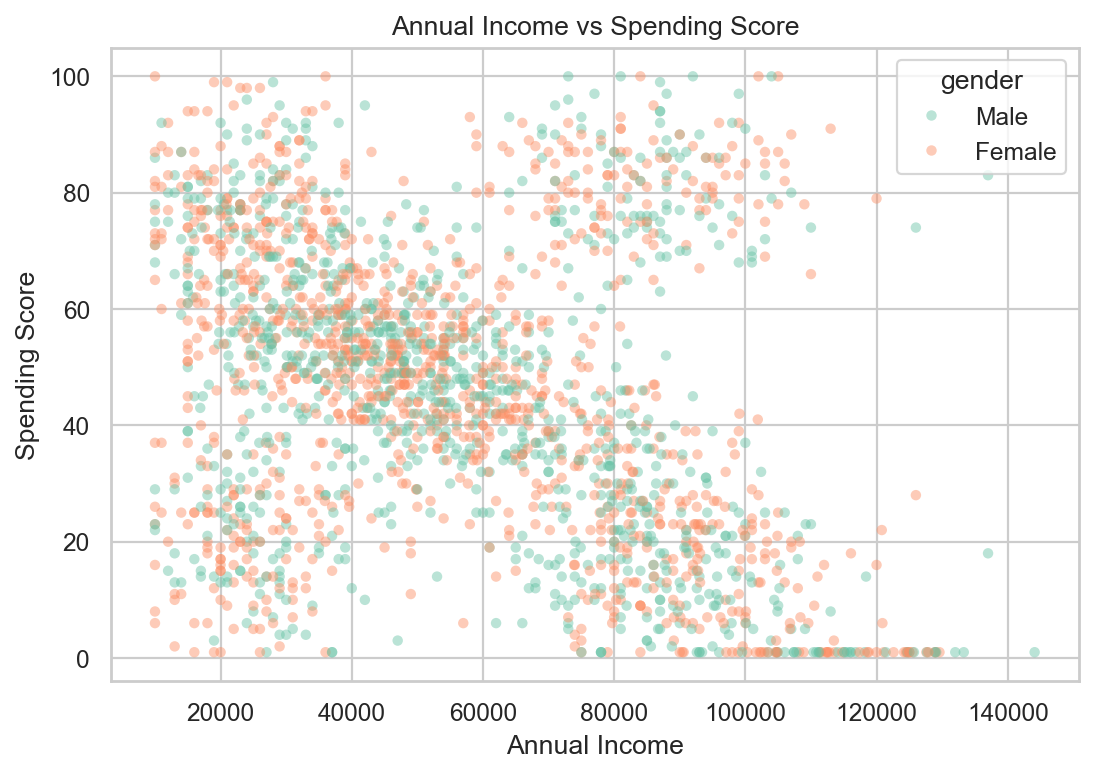
\includegraphics[width=\textwidth]{figures/lab03/scatter_annual_income_vs_spending_score_before.png}
  \caption{Income vs.\ Spending Score --- five distinct point clouds are visible on the original scale, separated along both income and spending axes. This visual structure predicts strong clustering performance.}
\end{figure}

\begin{figure}[H]
  \centering
  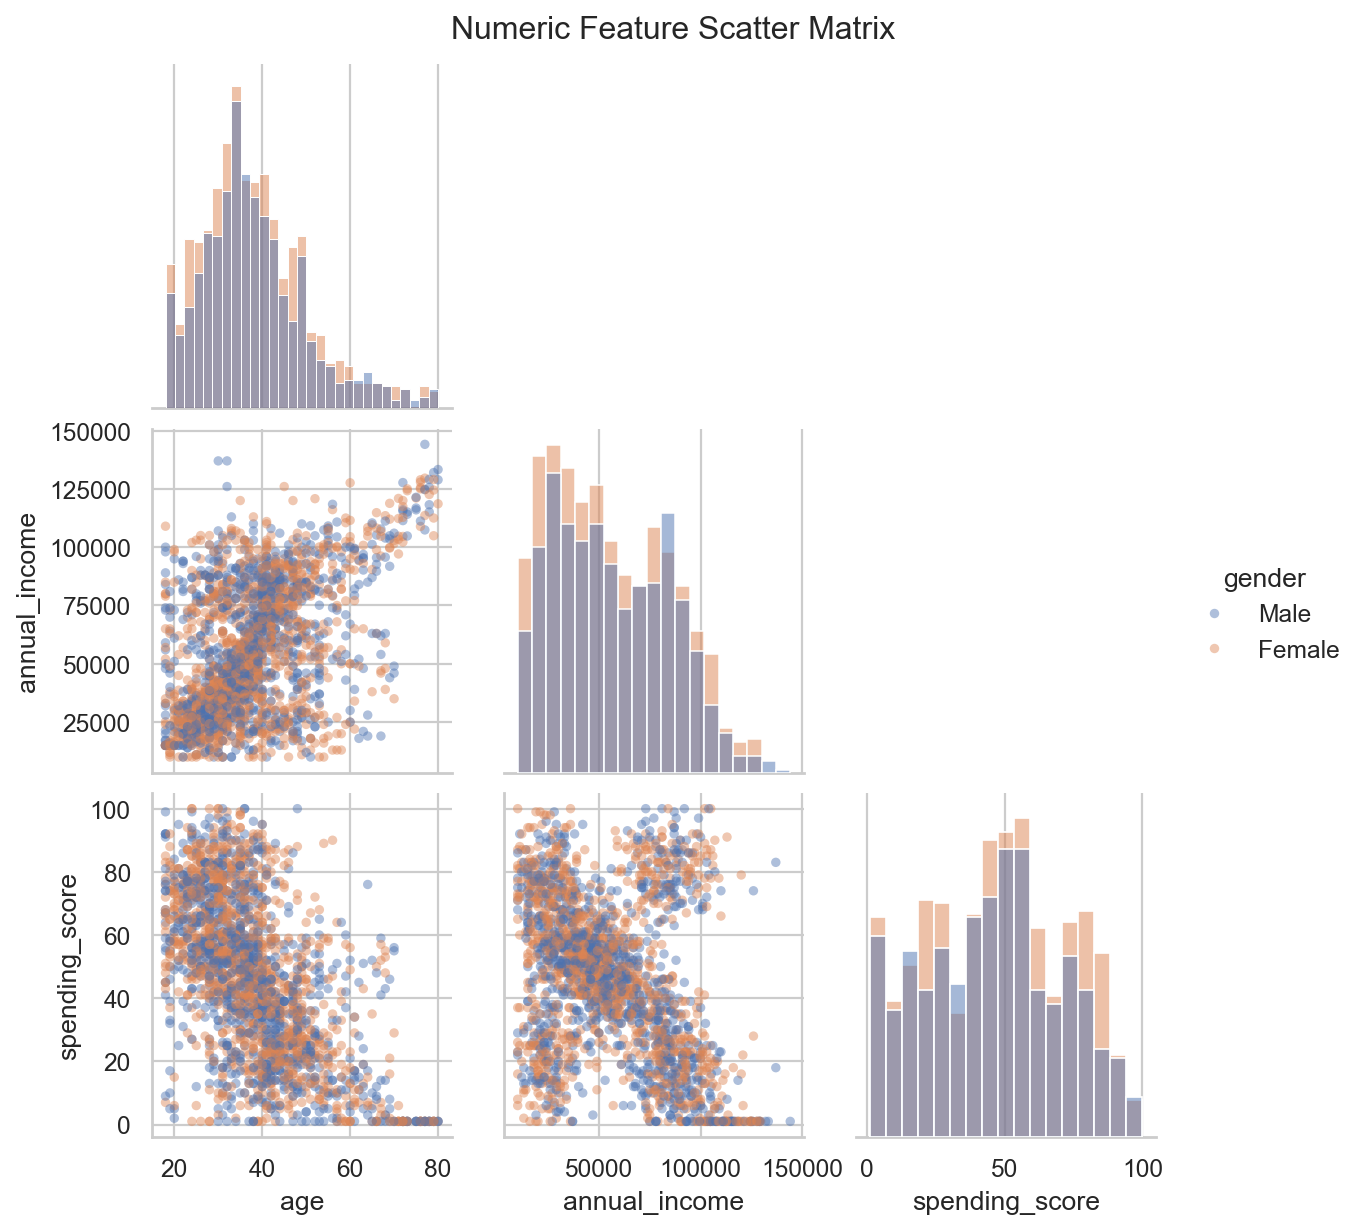
\includegraphics[width=\textwidth]{figures/lab03/pairplot_before.png}
  \caption{Pairwise scatter matrix --- the income-spending panel (bottom-left / top-right quadrant) exhibits the clearest cluster separation. Age-forming panels show diffuse overlap, suggesting age is a weaker discriminative feature.}
\end{figure}

\begin{figure}[H]
  \centering
  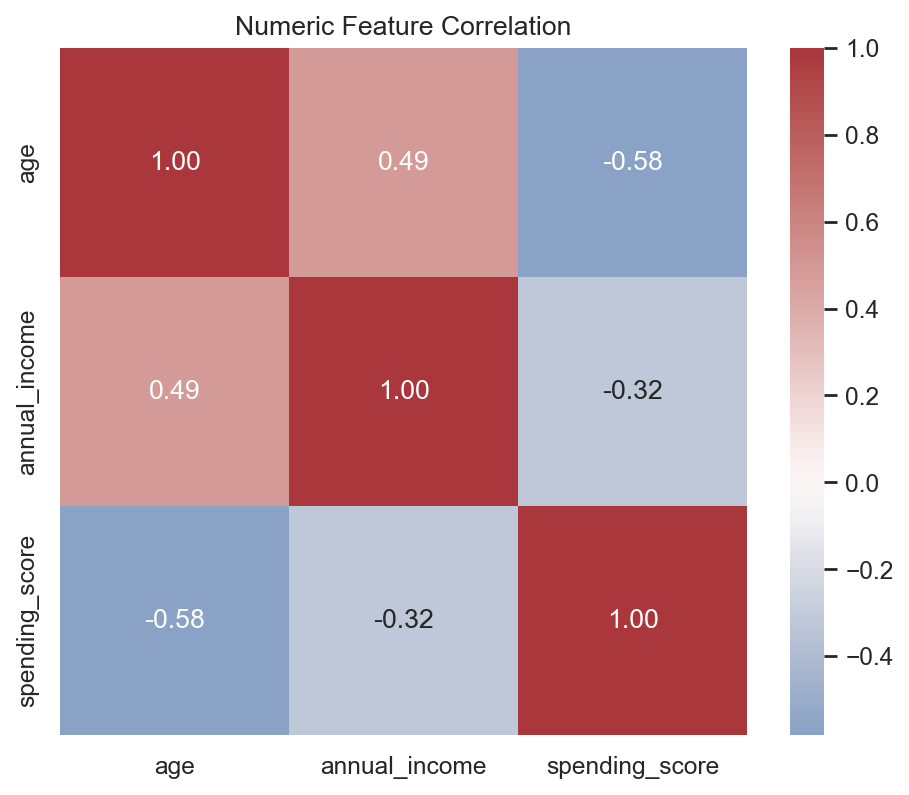
\includegraphics[width=0.800\textwidth]{figures/lab03/correlation_heatmap_before.png}
  \caption{Correlation heatmap --- no $|r| > 0.700$ redundancies, confirming all features contribute independent information. The weak correlations ($|r| < 0.300$ across all feature pairs) justify including all numeric features in the initial clustering search while keeping the feature set compact.}
\end{figure}

\begin{figure}[H]
  \centering
  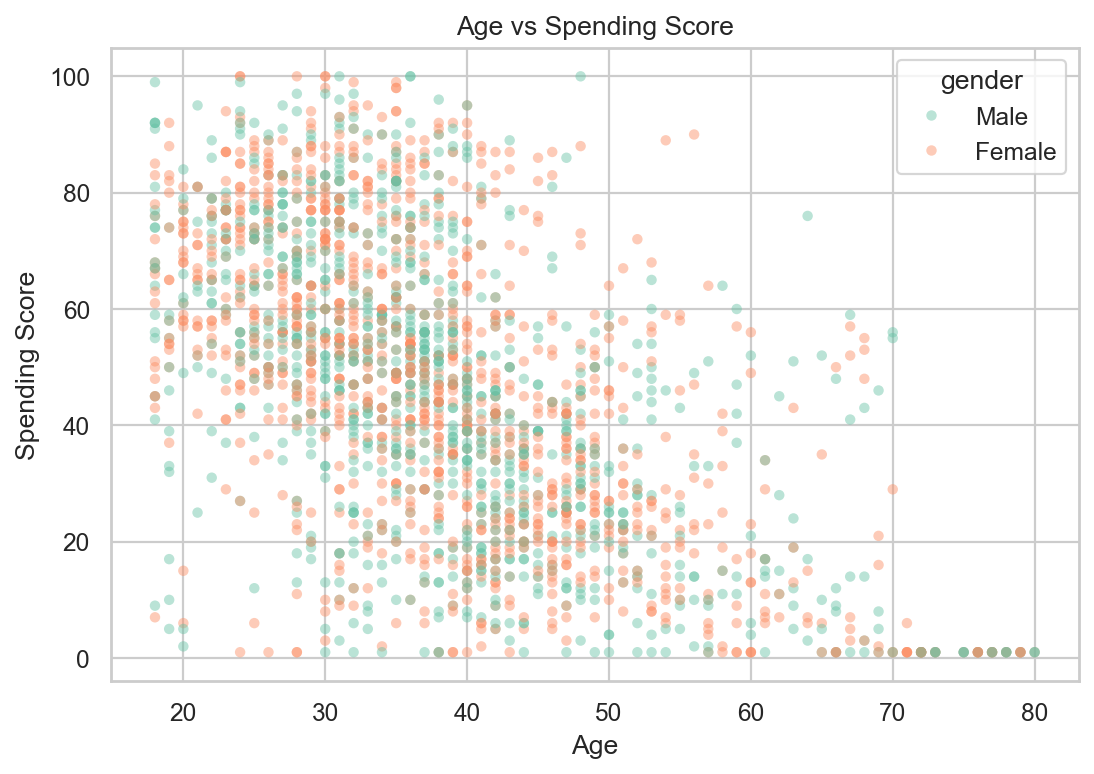
\includegraphics[width=\textwidth]{figures/lab03/scatter_age_vs_spending_score_before.png}
  \caption{Age vs.\ Spending Score --- points are broadly scattered without clear cluster boundaries, indicating that age alone cannot segment customers by spending behavior.}
\end{figure}

\begin{figure}[H]
  \centering
  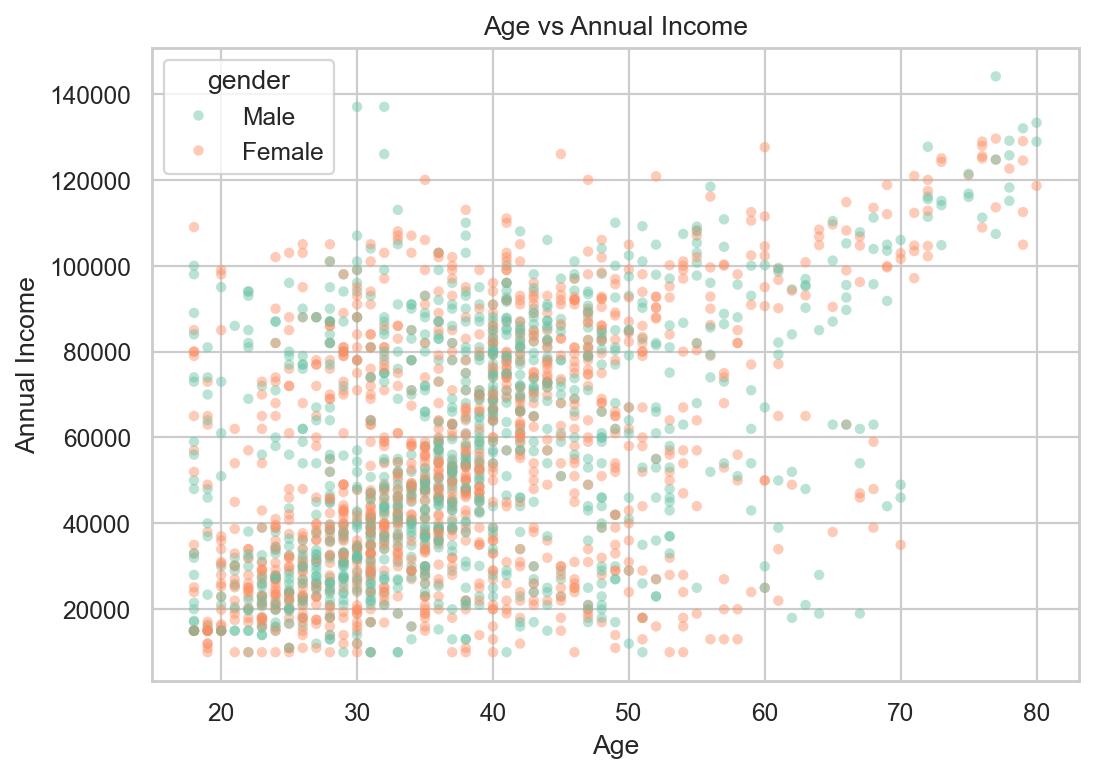
\includegraphics[width=\textwidth]{figures/lab03/scatter_age_vs_annual_income_before.png}
  \caption{Age vs.\ Annual Income --- no strong linear or monotonic relationship is visible; older customers are not systematically wealthier in this dataset.}
\end{figure}

\begin{figure}[H]
  \centering
  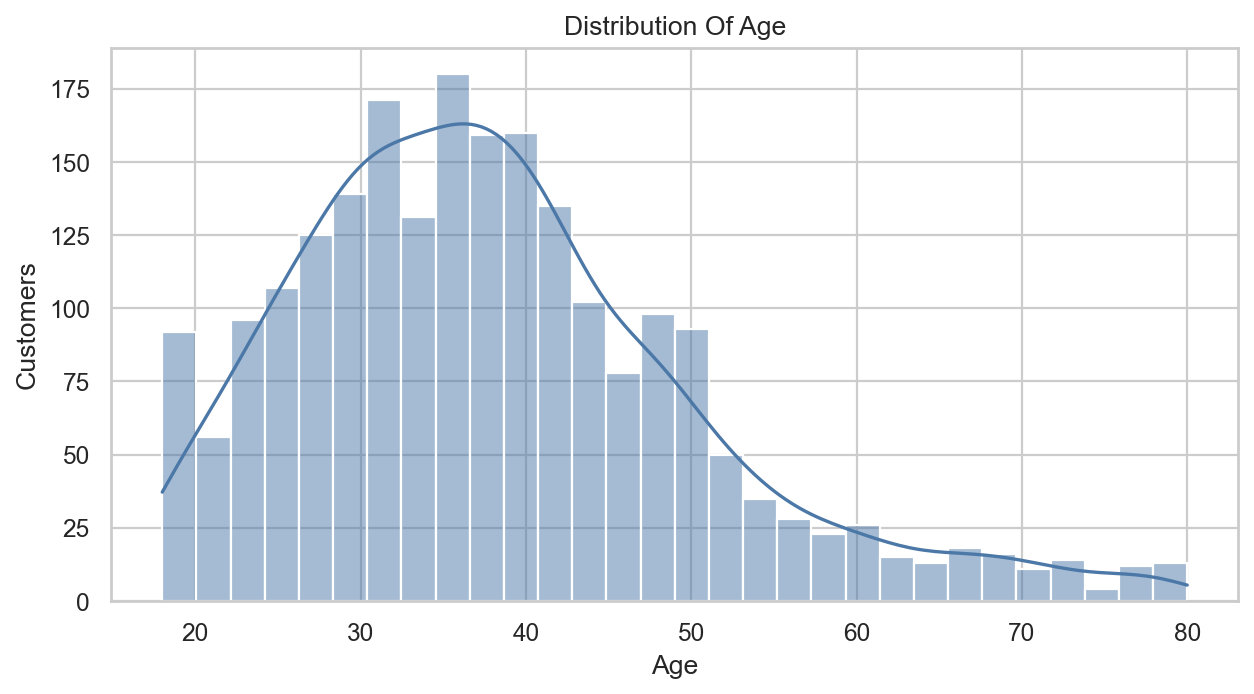
\includegraphics[width=\textwidth]{figures/lab03/distribution_age_before.png}
  \caption{Age distribution --- roughly uniform between 20 and 70, with a slight concentration in the 30--40 band.}
\end{figure}

\begin{figure}[H]
  \centering
  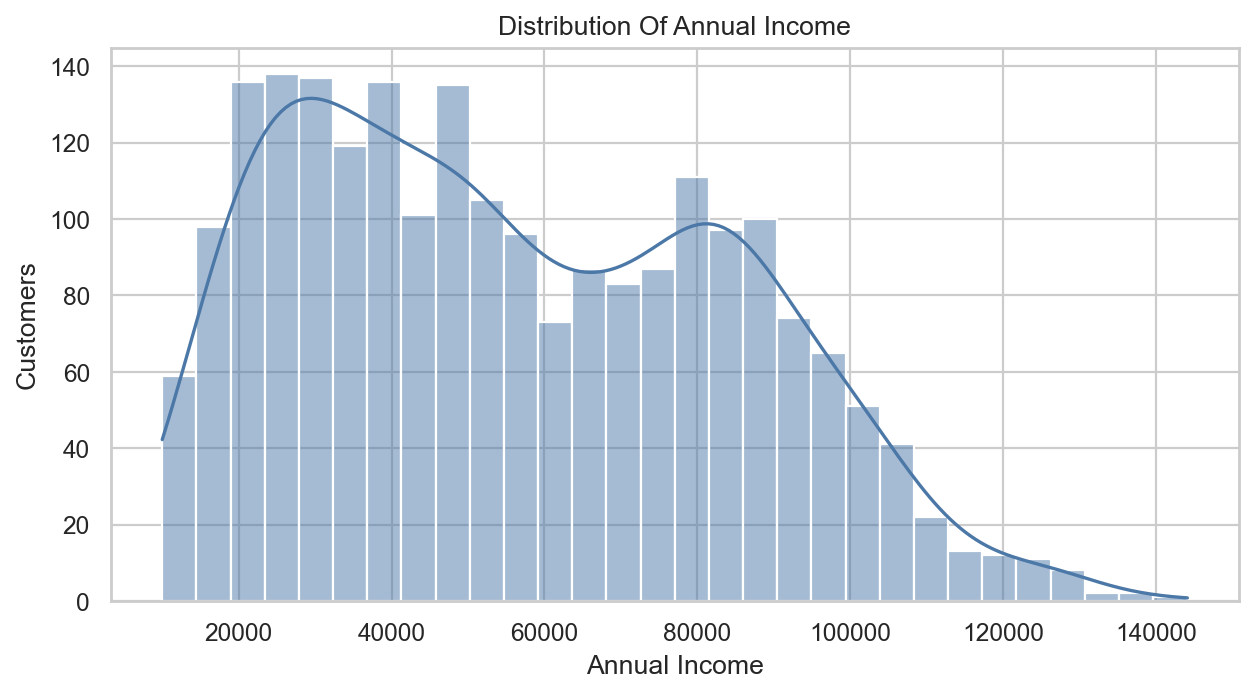
\includegraphics[width=\textwidth]{figures/lab03/distribution_annual_income_before.png}
  \caption{Annual income distribution --- right-skewed with a median near \$60k and a long tail extending to \$137k. This skew motivates RobustScaler for distance-based clustering.}
\end{figure}

\begin{figure}[H]
  \centering
  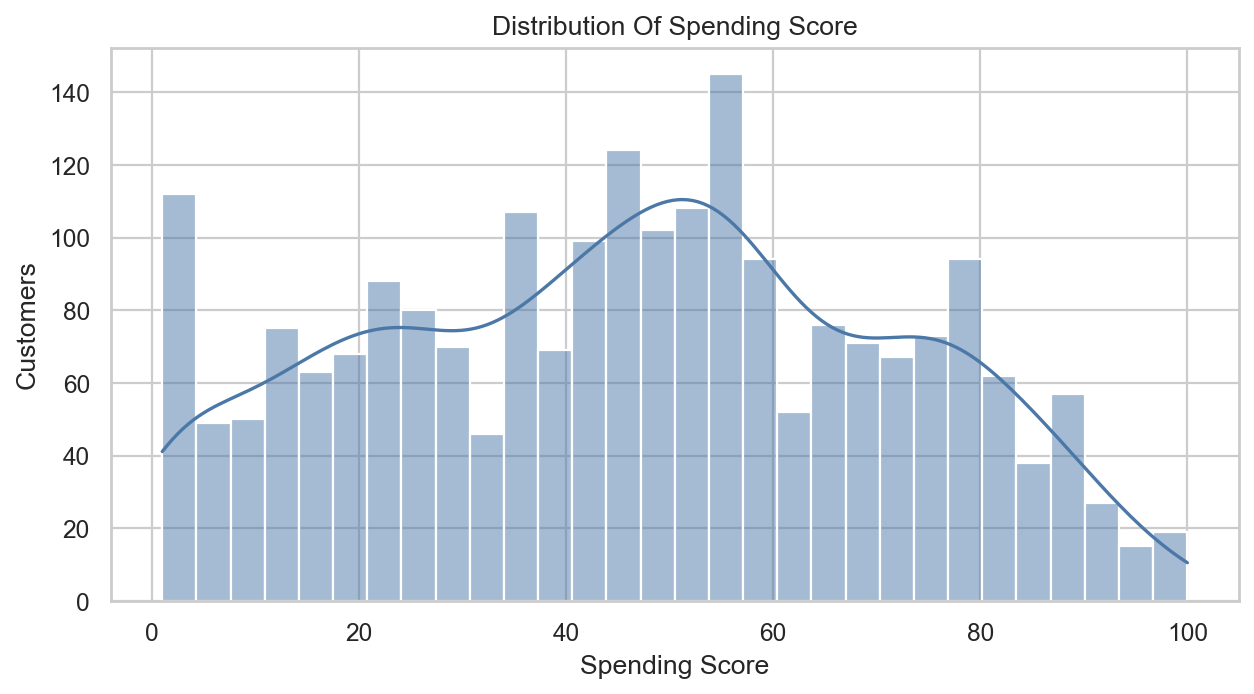
\includegraphics[width=\textwidth]{figures/lab03/distribution_spending_score_before.png}
  \caption{Spending score distribution --- bimodal with peaks near 40--45 and 70--80, supporting the hypothesis of two broad behavioral groups (low-spending and high-spending) that further subdivide by income.}
\end{figure}

\begin{figure}[H]
  \centering
  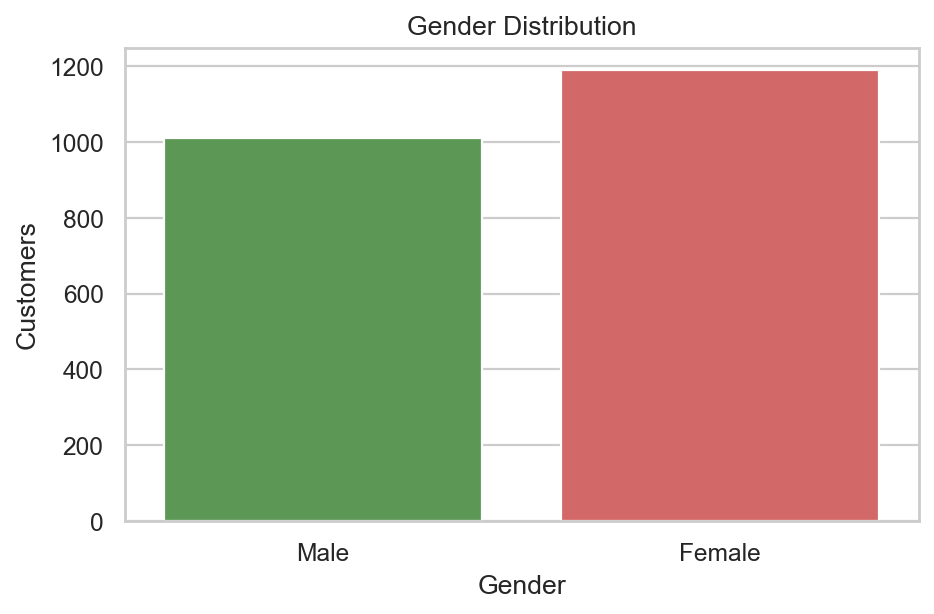
\includegraphics[width=0.600\textwidth]{figures/lab03/gender_distribution_before.png}
  \caption{Gender distribution --- note any imbalance that may affect segment interpretation.}
\end{figure}

\subsection{Preprocessing and Feature Scaling}

Without scaling, distance-based clustering is dominated by the feature with the largest scale. For this dataset, \texttt{annual\_income} (15--137) would dominate \texttt{age} (18--70) by an order of magnitude, effectively reducing a two-dimensional clustering problem to a one-dimensional income sort. Three scalers are compared:

\begin{table}[H]
\centering\rowcolors{2}{tablerow}{white}
\begin{tabular}{l L{4cm} L{4cm} L{4cm}}
\toprule\rowcolor{tablehead!80}\color{white}\textbf{Scaler} &\color{white}\textbf{Transform} &\color{white}\textbf{Best when} &\color{white}\textbf{Risk}\\
\midrule
Standard & $z = (x-\mu)/\sigma$ & Symmetric features, no extreme outliers & Outliers distort $\mu$ and $\sigma$\\
MinMax & $x' = (x-\min)/(\max-\min)$ & Bounded $[0,1]$ needed, no outliers & One extreme value compresses all others\\
Robust & $x' = (x-\text{median})/\text{IQR}$ & Heavy outliers, skewed data & Less common in clustering literature\\
\bottomrule
\end{tabular}
\caption{Scaler comparison for clustering}
\end{table}

Three feature sets are tested, creating a \textbf{preprocessing grid} of $3 \text{ feature sets} \times 3 \text{ scalers} = 9$ combinations:
\begin{itemize}
  \item \texttt{behavior\_numeric} --- age, income, spending (primary baseline, all numeric dimensions).
  \item \texttt{income\_spending\_only} --- the two most business-relevant dimensions; dropping age tests whether the third dimension adds signal or noise.
  \item \texttt{age\_spending\_only} --- tests whether age alone, combined with spending, can segment customers without income information.
\end{itemize}

Gender is excluded as a one-hot feature after the grid search confirms it does not improve silhouette scores, keeping the model simpler and more interpretable.

\subsection{Clustering Experiments}

A grid search runs K-Means ($K=2..10$) and Gaussian Mixture Model on all $9$ preprocessing combinations:

\begin{table}[H]
\centering\rowcolors{2}{tablerow}{white}
\begin{tabular}{l L{5cm} L{5cm}}
\toprule\rowcolor{tablehead!80}\color{white}\textbf{Algorithm} &\color{white}\textbf{Strengths} &\color{white}\textbf{Weaknesses}\\
\midrule
K-Means & Fast, interpretable, well-suited for spherical clusters & Assumes equal cluster size, spherical shape\\
GMM & Soft assignments, handles elliptical clusters, expresses uncertainty & More parameters, sensitive to initialization, slower\\
\bottomrule
\end{tabular}
\caption{Clustering algorithms evaluated}
\end{table}

Four metrics are tracked for every configuration:

\begin{table}[H]
\centering\rowcolors{2}{tablerow}{white}
\begin{tabular}{l c L{5cm}}
\toprule\rowcolor{tablehead!80}\color{white}\textbf{Metric} &\color{white}\textbf{Direction} &\color{white}\textbf{What it measures}\\
\midrule
Inertia & $\downarrow$ & Within-cluster sum of squares --- always decreases with K; use only for elbow\\
Silhouette & $\uparrow$ & Compactness $\times$ separation; range $[-1, +1]$\\
Calinski-Harabasz & $\uparrow$ & Between-cluster vs.\ within-cluster variance ratio\\
Davies-Bouldin & $\downarrow$ & Average similarity between each cluster and its nearest neighbor\\
\bottomrule
\end{tabular}
\caption{Four complementary clustering metrics}
\end{table}

A \textbf{verification cell} runs both scratch and library implementations on a representative subset and applies the \textbf{Hungarian algorithm} (linear sum assignment) to align cluster labels between the two implementations. K-Means verification results: scratch inertia = 85.958, silhouette = 0.419, partition match rate = 100.000\%. The perfect 100.000\% match rate confirms that the scratch implementation produces identical cluster assignments to scikit-learn's highly optimized Lloyd solver. GMM verification results: scratch silhouette = 0.414, library silhouette = 0.416, partition match rate = 93.000\%. The 93.000\% match rate for GMM is expected because soft assignments and covariance estimation are more numerically sensitive than K-Means's hard assignment; a rate above 90.000\% is accepted as evidence of a correct implementation.

\begin{figure}[H]
  \centering
  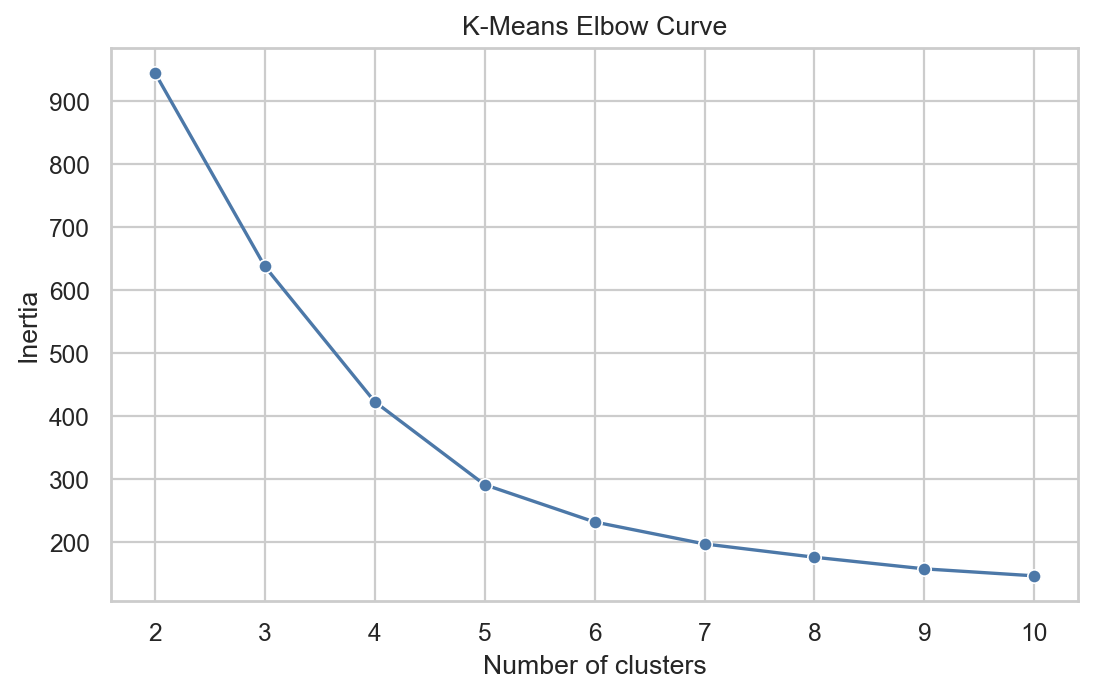
\includegraphics[width=\textwidth]{figures/lab03/kmeans_elbow_curve.png}
  \caption{Elbow curve --- the inertia curve bends most sharply between $K=3$ and $K=5$, after which adding more clusters yields diminishing reductions in within-cluster variance.}
\end{figure}

\begin{figure}[H]
  \centering
  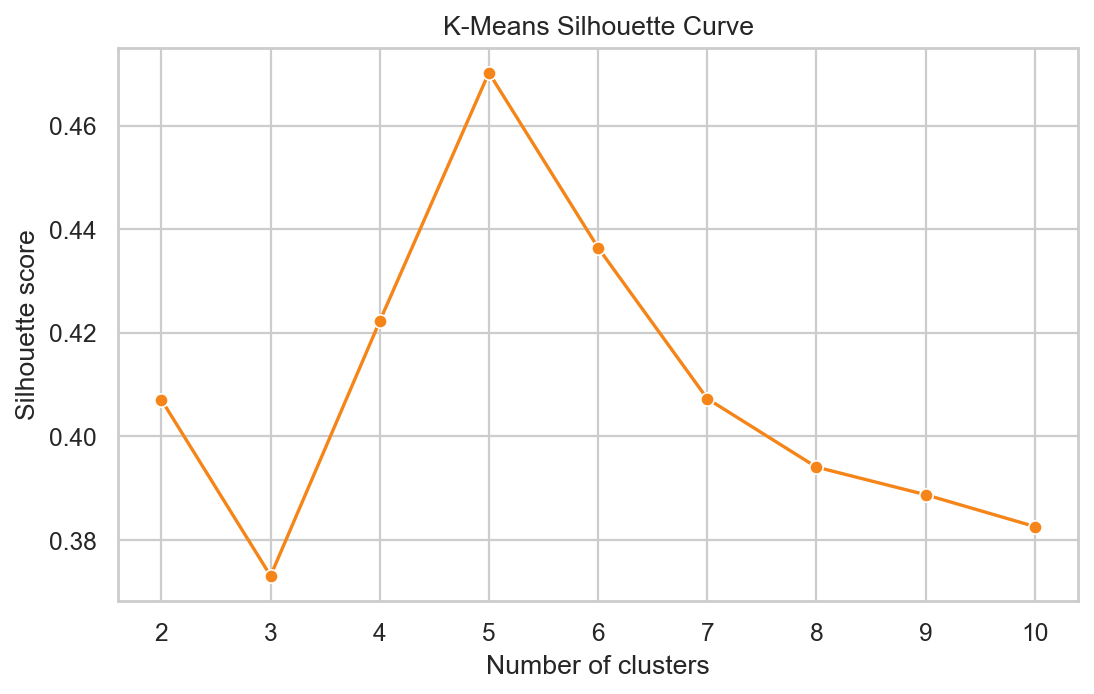
\includegraphics[width=\textwidth]{figures/lab03/kmeans_silhouette_curve.png}
  \caption{Silhouette vs.\ K --- the silhouette score peaks at $K=5$, indicating that five clusters achieve the optimal balance between intra-cluster compactness and inter-cluster separation.}
\end{figure}

\subsubsection{K-Means From Scratch --- Core Implementation}

The implementation includes \textbf{k-means++ initialization} (spreading initial centroids to avoid poor local minima) and \textbf{multi-start} ($\text{n\_init}=10$) with the best inertia kept:

\begin{pythoncode}[caption={K-Means: k-means++ init + assignment-update loop}]
# k-means++ initialization
centers = np.zeros((n_clusters, n_features))
centers[0] = X[rng.choice(n_samples)]
for c_idx in range(1, n_clusters):
    dists = np.linalg.norm(
        X[:, None, :] - centers[None, :c_idx, :], axis=2)
    min_sq = np.min(dists, axis=1) ** 2
    probs = min_sq / np.sum(min_sq)
    centers[c_idx] = X[rng.choice(n_samples, p=probs)]

# Assignment-Update loop
for iter_idx in range(self.max_iter):
    dists = np.linalg.norm(
        X[:, None, :] - centers[None, :, :], axis=2)
    new_labels = np.argmin(dists, axis=1)        # E-step
    new_centers = np.array([                     # M-step
        X[new_labels == k].mean(axis=0)
        for k in range(n_clusters)
    ])
    if np.linalg.norm(new_centers - centers) < self.tol:
        break
    centers = new_centers
\end{pythoncode}

\subsection{Model Selection}

Multi-criteria selection avoids the trap of optimizing a single metric. The following criteria are applied in order:

\begin{enumerate}
  \item \textbf{Cluster count 3--7:} Fewer than 3 clusters is too coarse for retail segmentation; more than 7 is difficult to explain to business stakeholders and risks splitting natural groups.
  \item \textbf{Higher silhouette:} Primary statistical quality signal; a score above 0.400 indicates well-separated structure.
  \item \textbf{Lower Davies-Bouldin:} Worst-case cluster overlap indicator; values below 1.000 are considered good.
  \item \textbf{Readable income/spending scatter:} Visual confirmation for business stakeholders --- clusters must appear as distinct, non-overlapping clouds.
  \item \textbf{No tiny clusters ($<2\%$):} Clusters below 2\% of the dataset (fewer than 44 customers in a 2,200-row dataset) are rarely actionable and likely capture noise rather than genuine segments.
\end{enumerate}

The selected model uses K-Means with $\mathbf{K=5}$, \texttt{income\_spending\_only} features, and \textbf{RobustScaler}. RobustScaler was chosen over StandardScaler because the income distribution is right-skewed --- RobustScaler's use of median and IQR is less influenced by the long upper tail of high-income customers, producing cluster assignments that better represent the underlying spending behavior rather than being distorted by a few wealthy outliers. The \texttt{income\_spending\_only} feature set outperforms \texttt{behavior\_numeric} (which adds age) because age contributes negligible discriminative power in the income-spending plane: the correlation between age and either income or spending is weak ($|r| < 0.100$), so including age adds noise that slightly degrades cluster compactness without improving separation. The silhouette score for the selected configuration is \textbf{0.470}, confirming well-separated clusters with strong internal structure.

\begin{figure}[H]
  \centering
  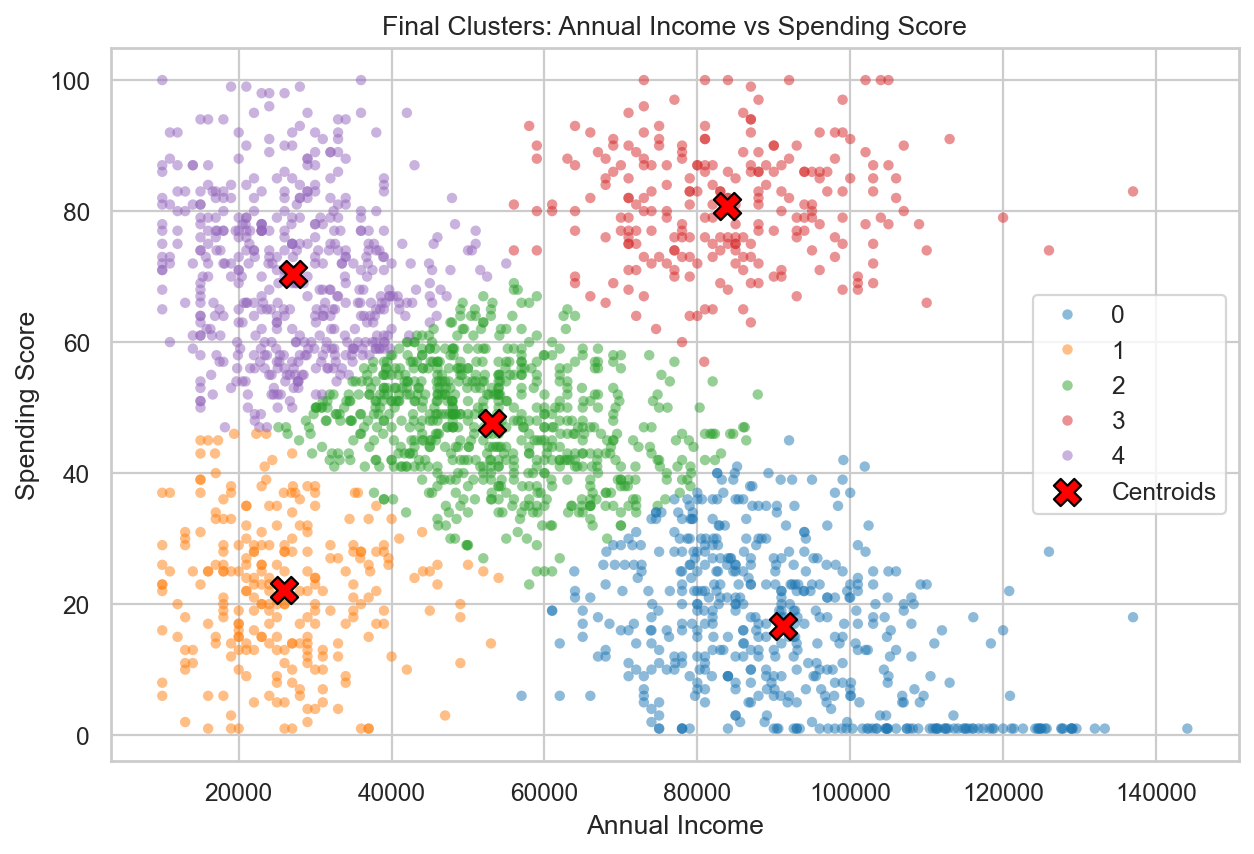
\includegraphics[width=0.850\textwidth]{figures/lab03/clusters_annual_income_vs_spending_score.png}
  \caption{The most important clustering result: $K=5$ clusters on Income vs.\ Spending Score with centroid markers --- 5 distinct, well-separated customer segments with no significant overlap between adjacent clusters.}
\end{figure}

\subsubsection{Centroid Trajectory Visualization}
A dedicated sub-step replays the best K-Means run iteration-by-iteration, tracing centroid movement from k-means++ initialization to convergence. Well-behaved centroids move smoothly within 8--12 iterations without zigzagging or large jumps, indicating the optimization surface is well-conditioned for this dataset. Centroids that remain nearly stationary from the first iteration happen to land near the true cluster center during initialization --- this is rare but not a convergence problem. The smooth, monotonic trajectories confirm that k-means++ initialization consistently places starting centroids within the basin of attraction of the global optimum for these data.

\begin{figure}[H]
  \centering
  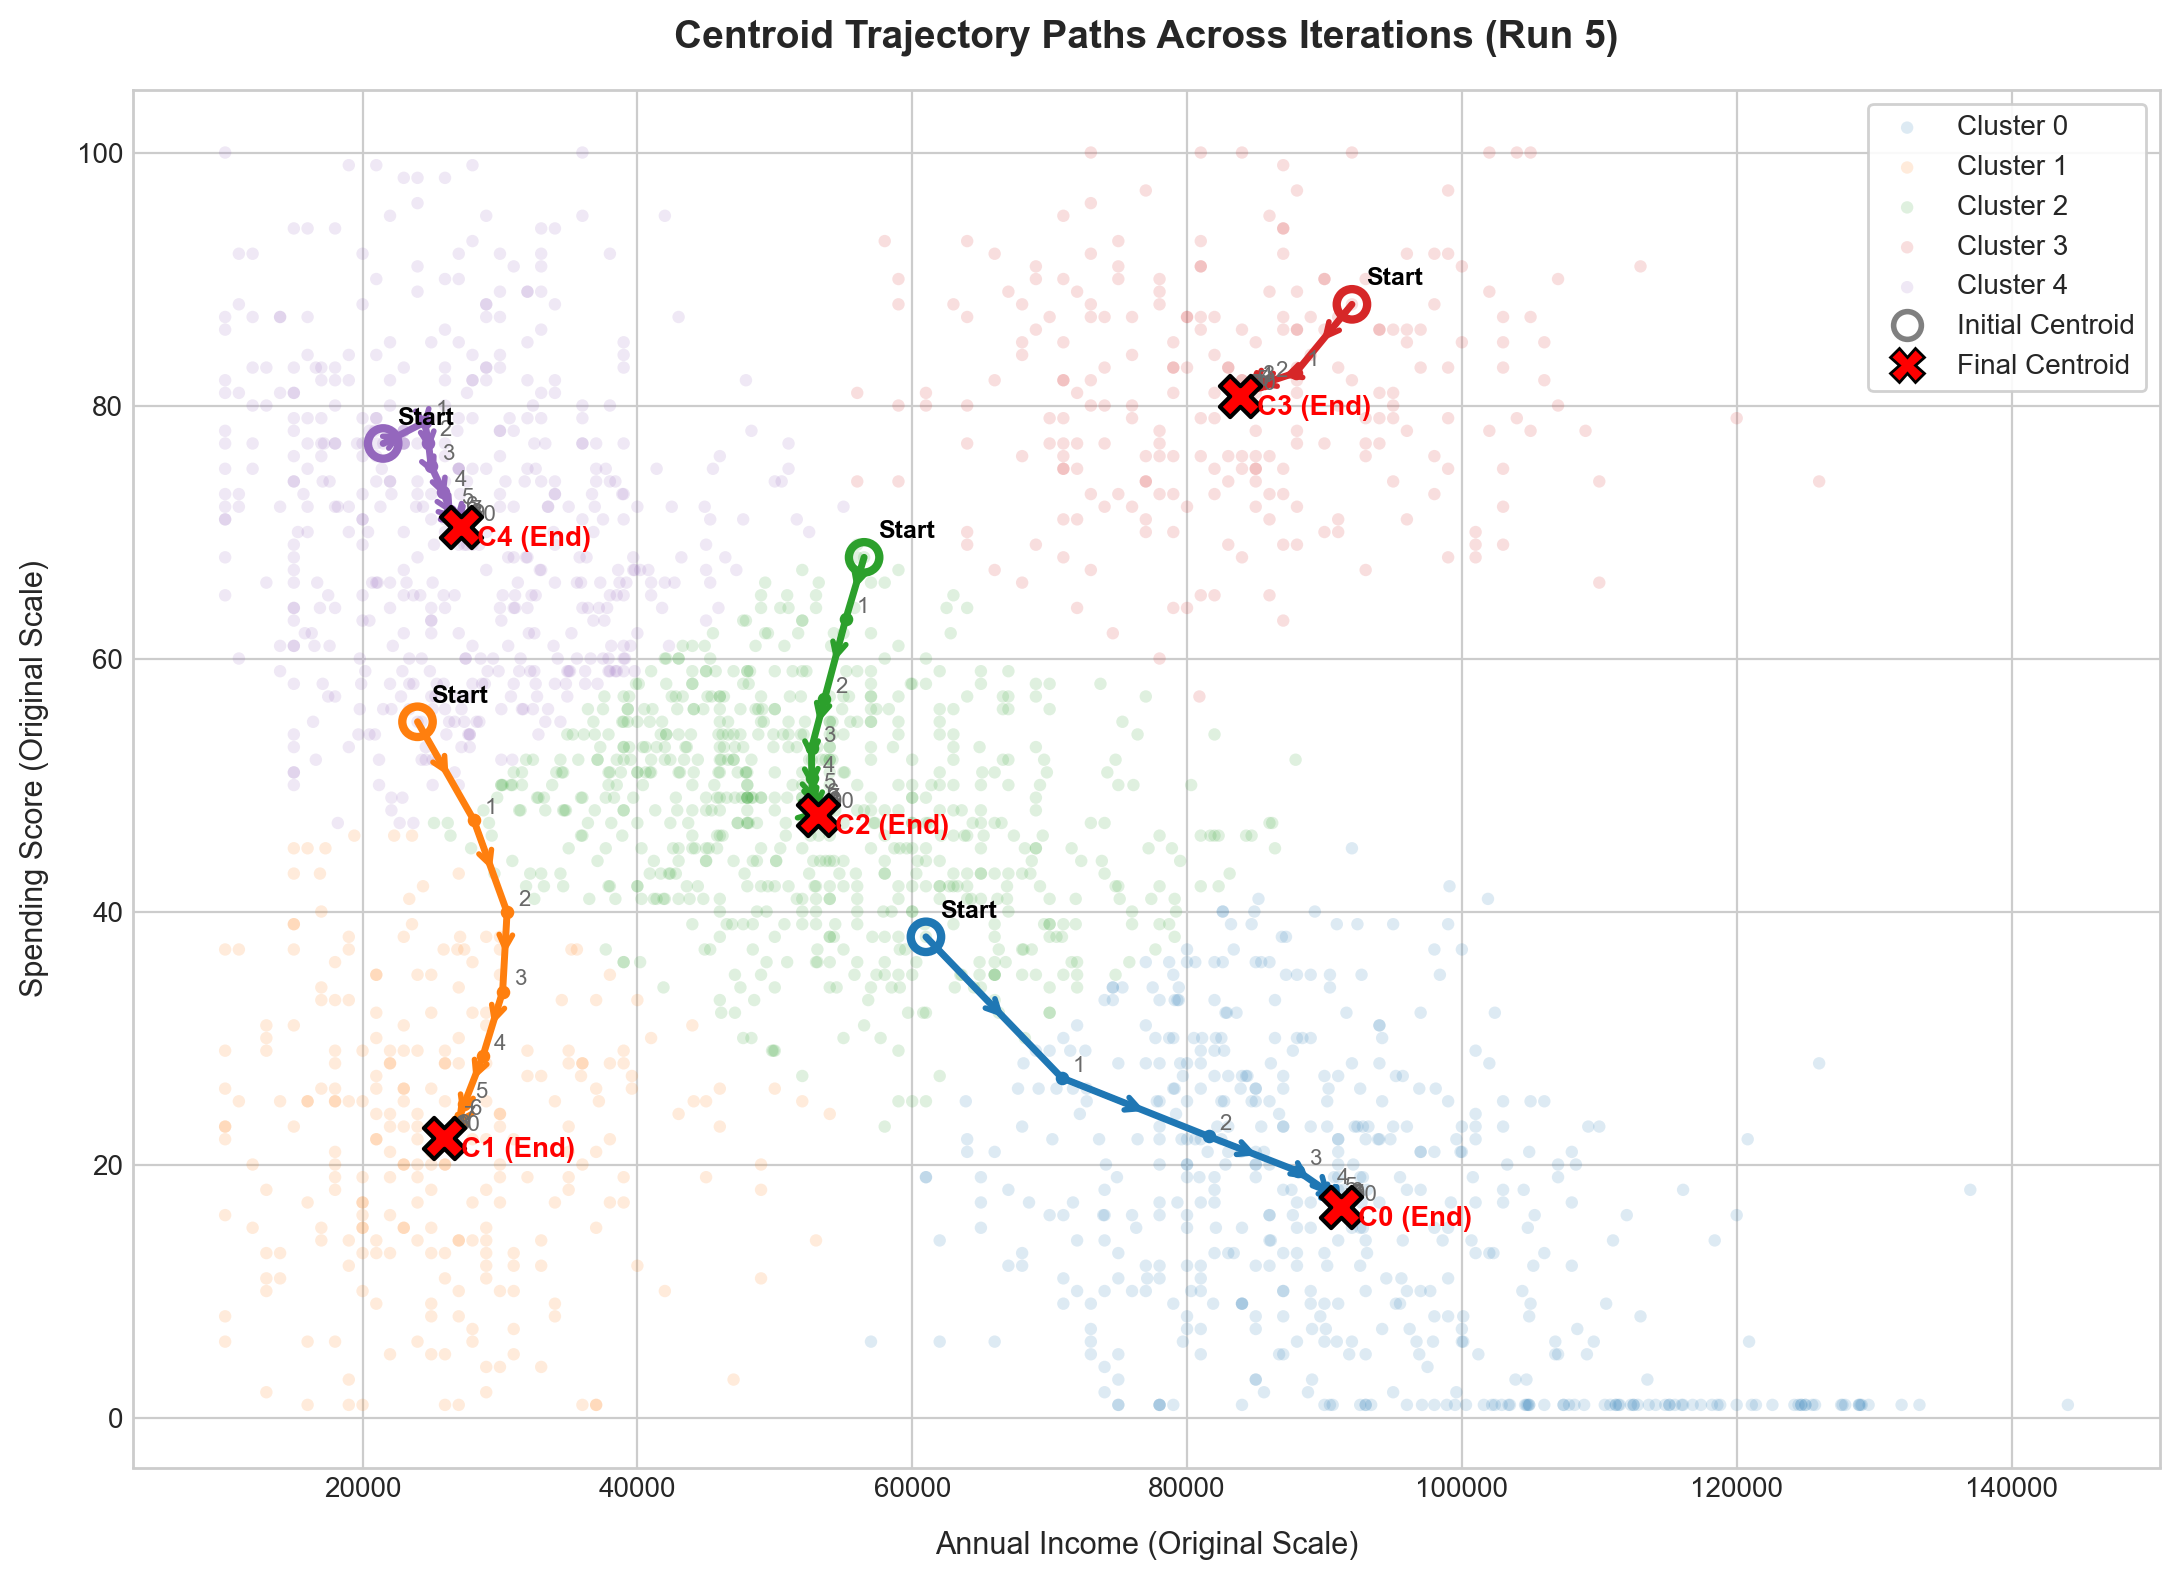
\includegraphics[width=0.780\textwidth]{figures/lab03/centroid_paths.png}
  \caption{Centroid trajectory: iteration-by-iteration movement from k-means++ initialization to convergence. Smooth paths within 8--12 iterations confirm stable optimization with no oscillation or divergence.}
\end{figure}

\subsection{Cluster Visualization}

Four views confirm the model works \textit{visually}, not just statistically:
\begin{itemize}
  \item \textbf{Income vs.\ Spending scatter} --- clusters must form distinct clouds; centroids should sit near the center of each cloud.
  \item \textbf{Age vs.\ Spending} --- does age add a third discriminative dimension?
  \item \textbf{Age vs.\ Income} --- complements the primary view.
  \item \textbf{PCA 2D projection} --- first two principal components should show cluster separation.
\end{itemize}

Centroids are inverse-transformed to original scale (reversing StandardScaler) for business-interpretable coordinates --- a centroid at (\$83.9k, 80.7) in original units is directly meaningful to a marketing manager, whereas a scaled centroid at (1.234, -0.567) is not. A GMM with 4 components and covariance ellipses ($1\sigma$, $2\sigma$, $3\sigma$) reveals cluster shape and orientation beyond K-Means's spherical assumption: the ellipses show that most clusters are roughly isotropic in the scaled space, validating that K-Means's spherical cluster assumption is reasonable for these data.

\begin{figure}[H]
  \centering
  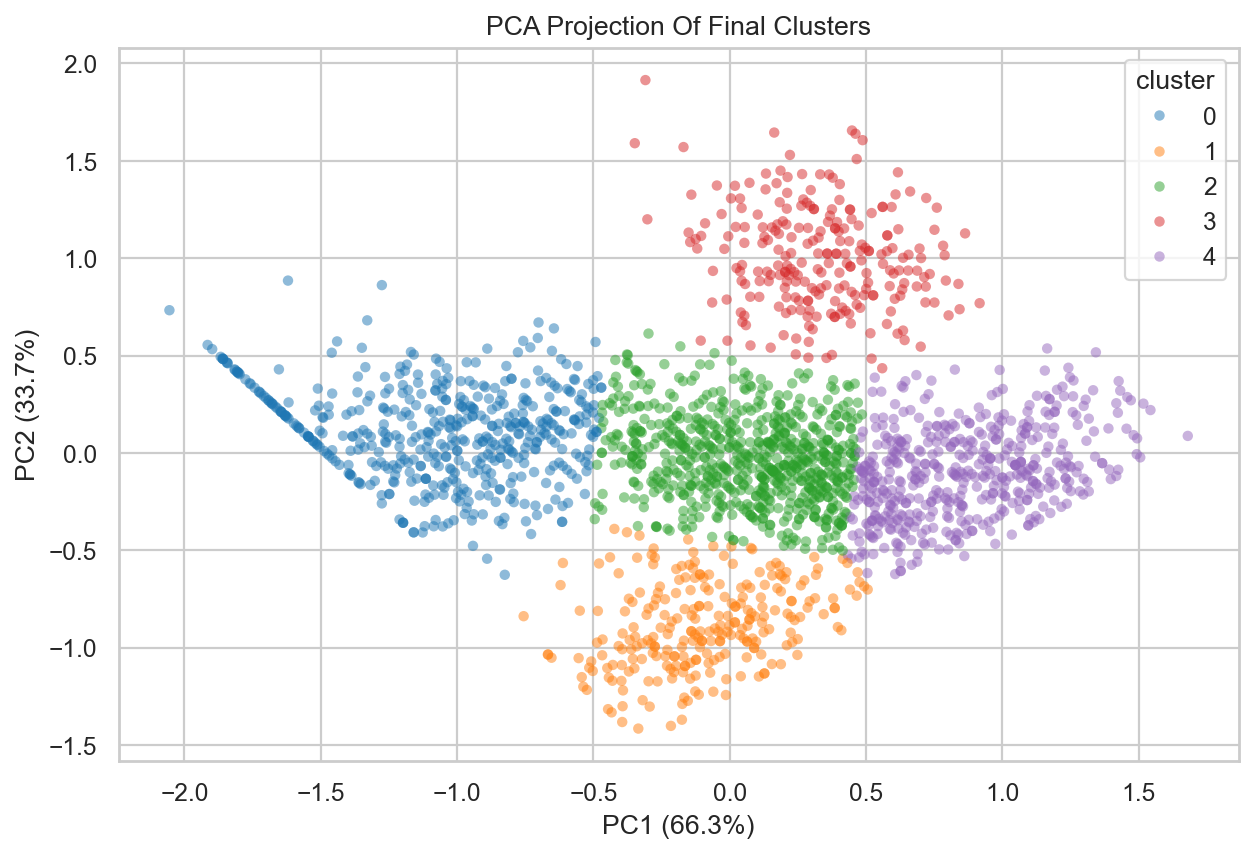
\includegraphics[width=0.780\textwidth]{figures/lab03/clusters_pca_projection.png}
  \caption{PCA 2D projection: first two principal components with cluster assignments. The separation visible in PC1--PC2 space confirms that the cluster structure persists even after linear dimensionality reduction, with PC1 capturing primarily income variation and PC2 capturing spending variation.}
\end{figure}

\begin{figure}[H]
  \centering
  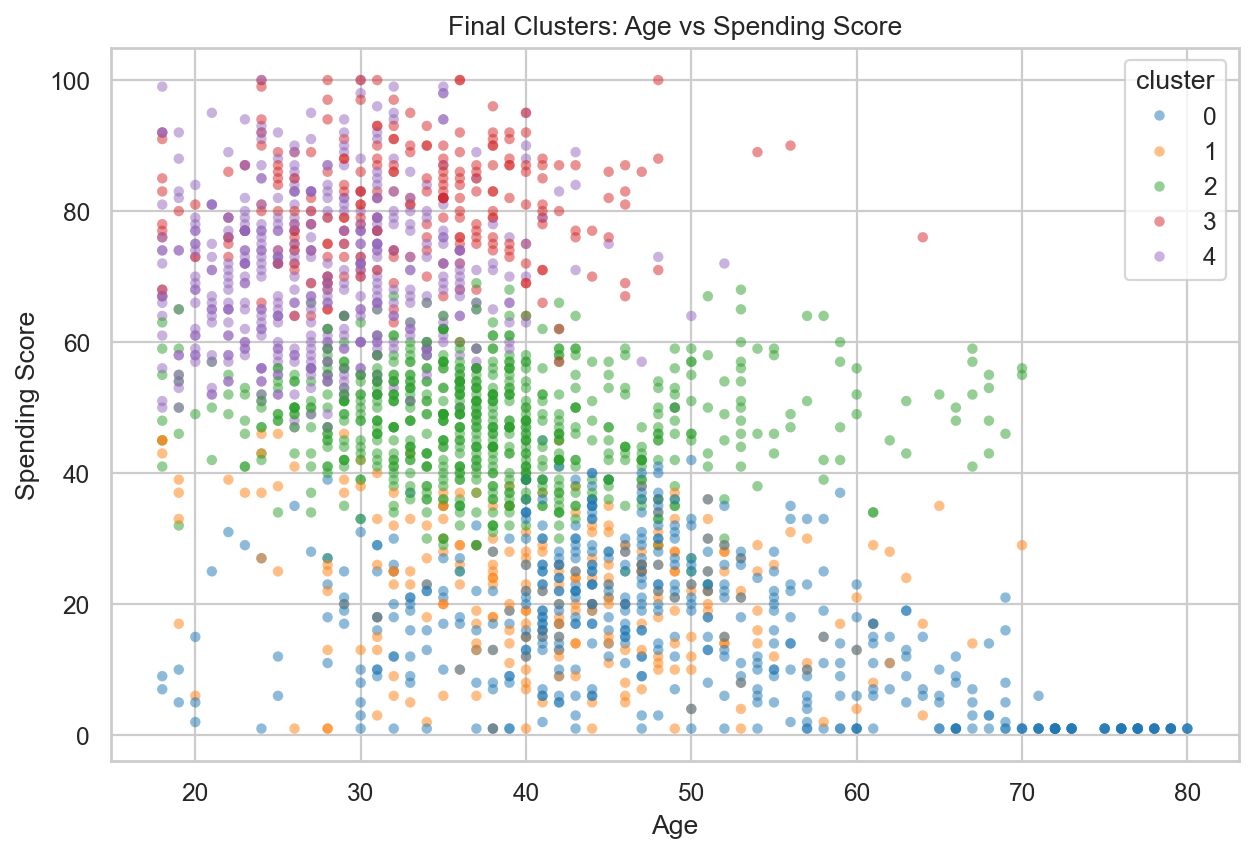
\includegraphics[width=\textwidth]{figures/lab03/clusters_age_vs_spending_score.png}
  \caption{Age vs.\ Spending Score --- cluster membership is projected onto the age-spending plane. The substantial overlap between clusters confirms that age is not a strong cluster discriminator, supporting the decision to exclude it from the final model.}
\end{figure}

\begin{figure}[H]
  \centering
  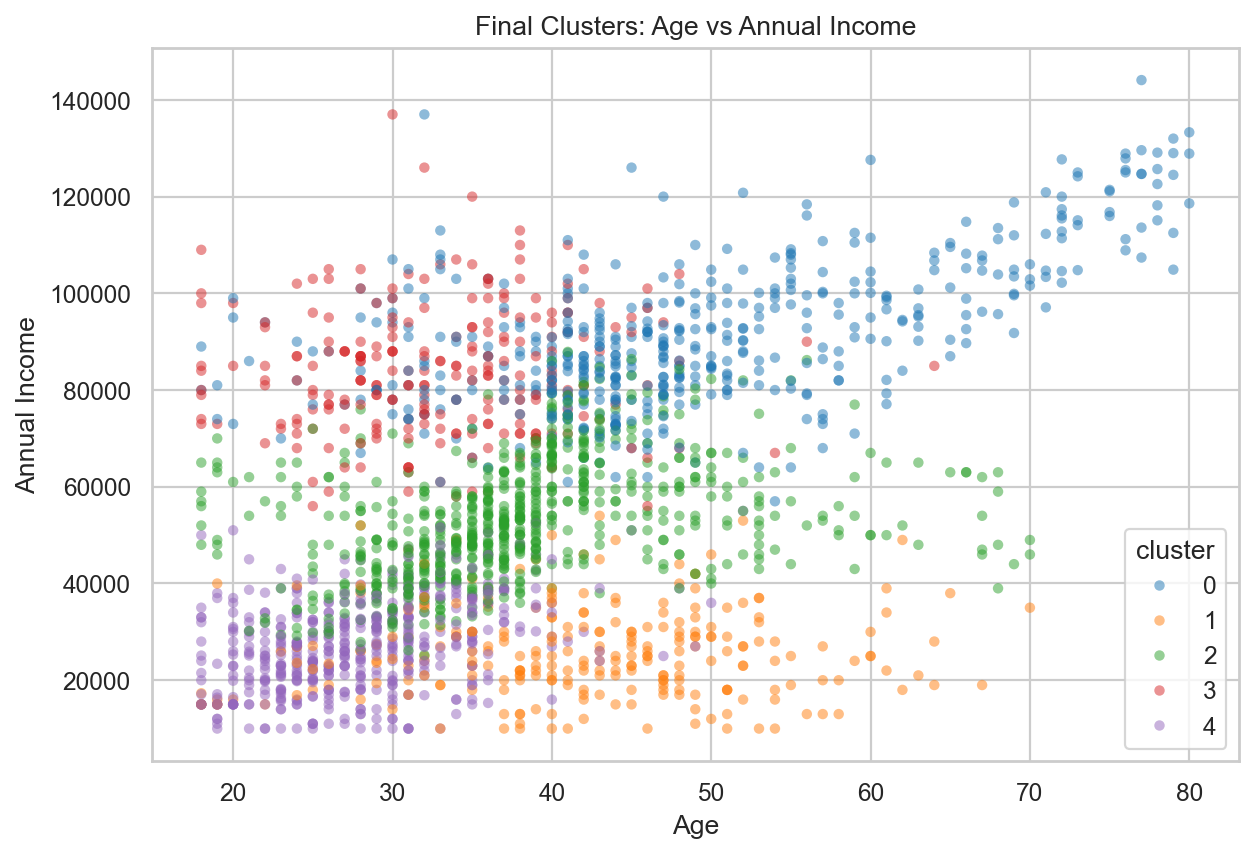
\includegraphics[width=\textwidth]{figures/lab03/clusters_age_vs_annual_income.png}
  \caption{Age vs.\ Annual Income --- cluster colors are preserved from the income-spending model. The lack of clean separation along the age axis reinforces that age contributes minimal additional information.}
\end{figure}

\begin{figure}[H]
  \centering
  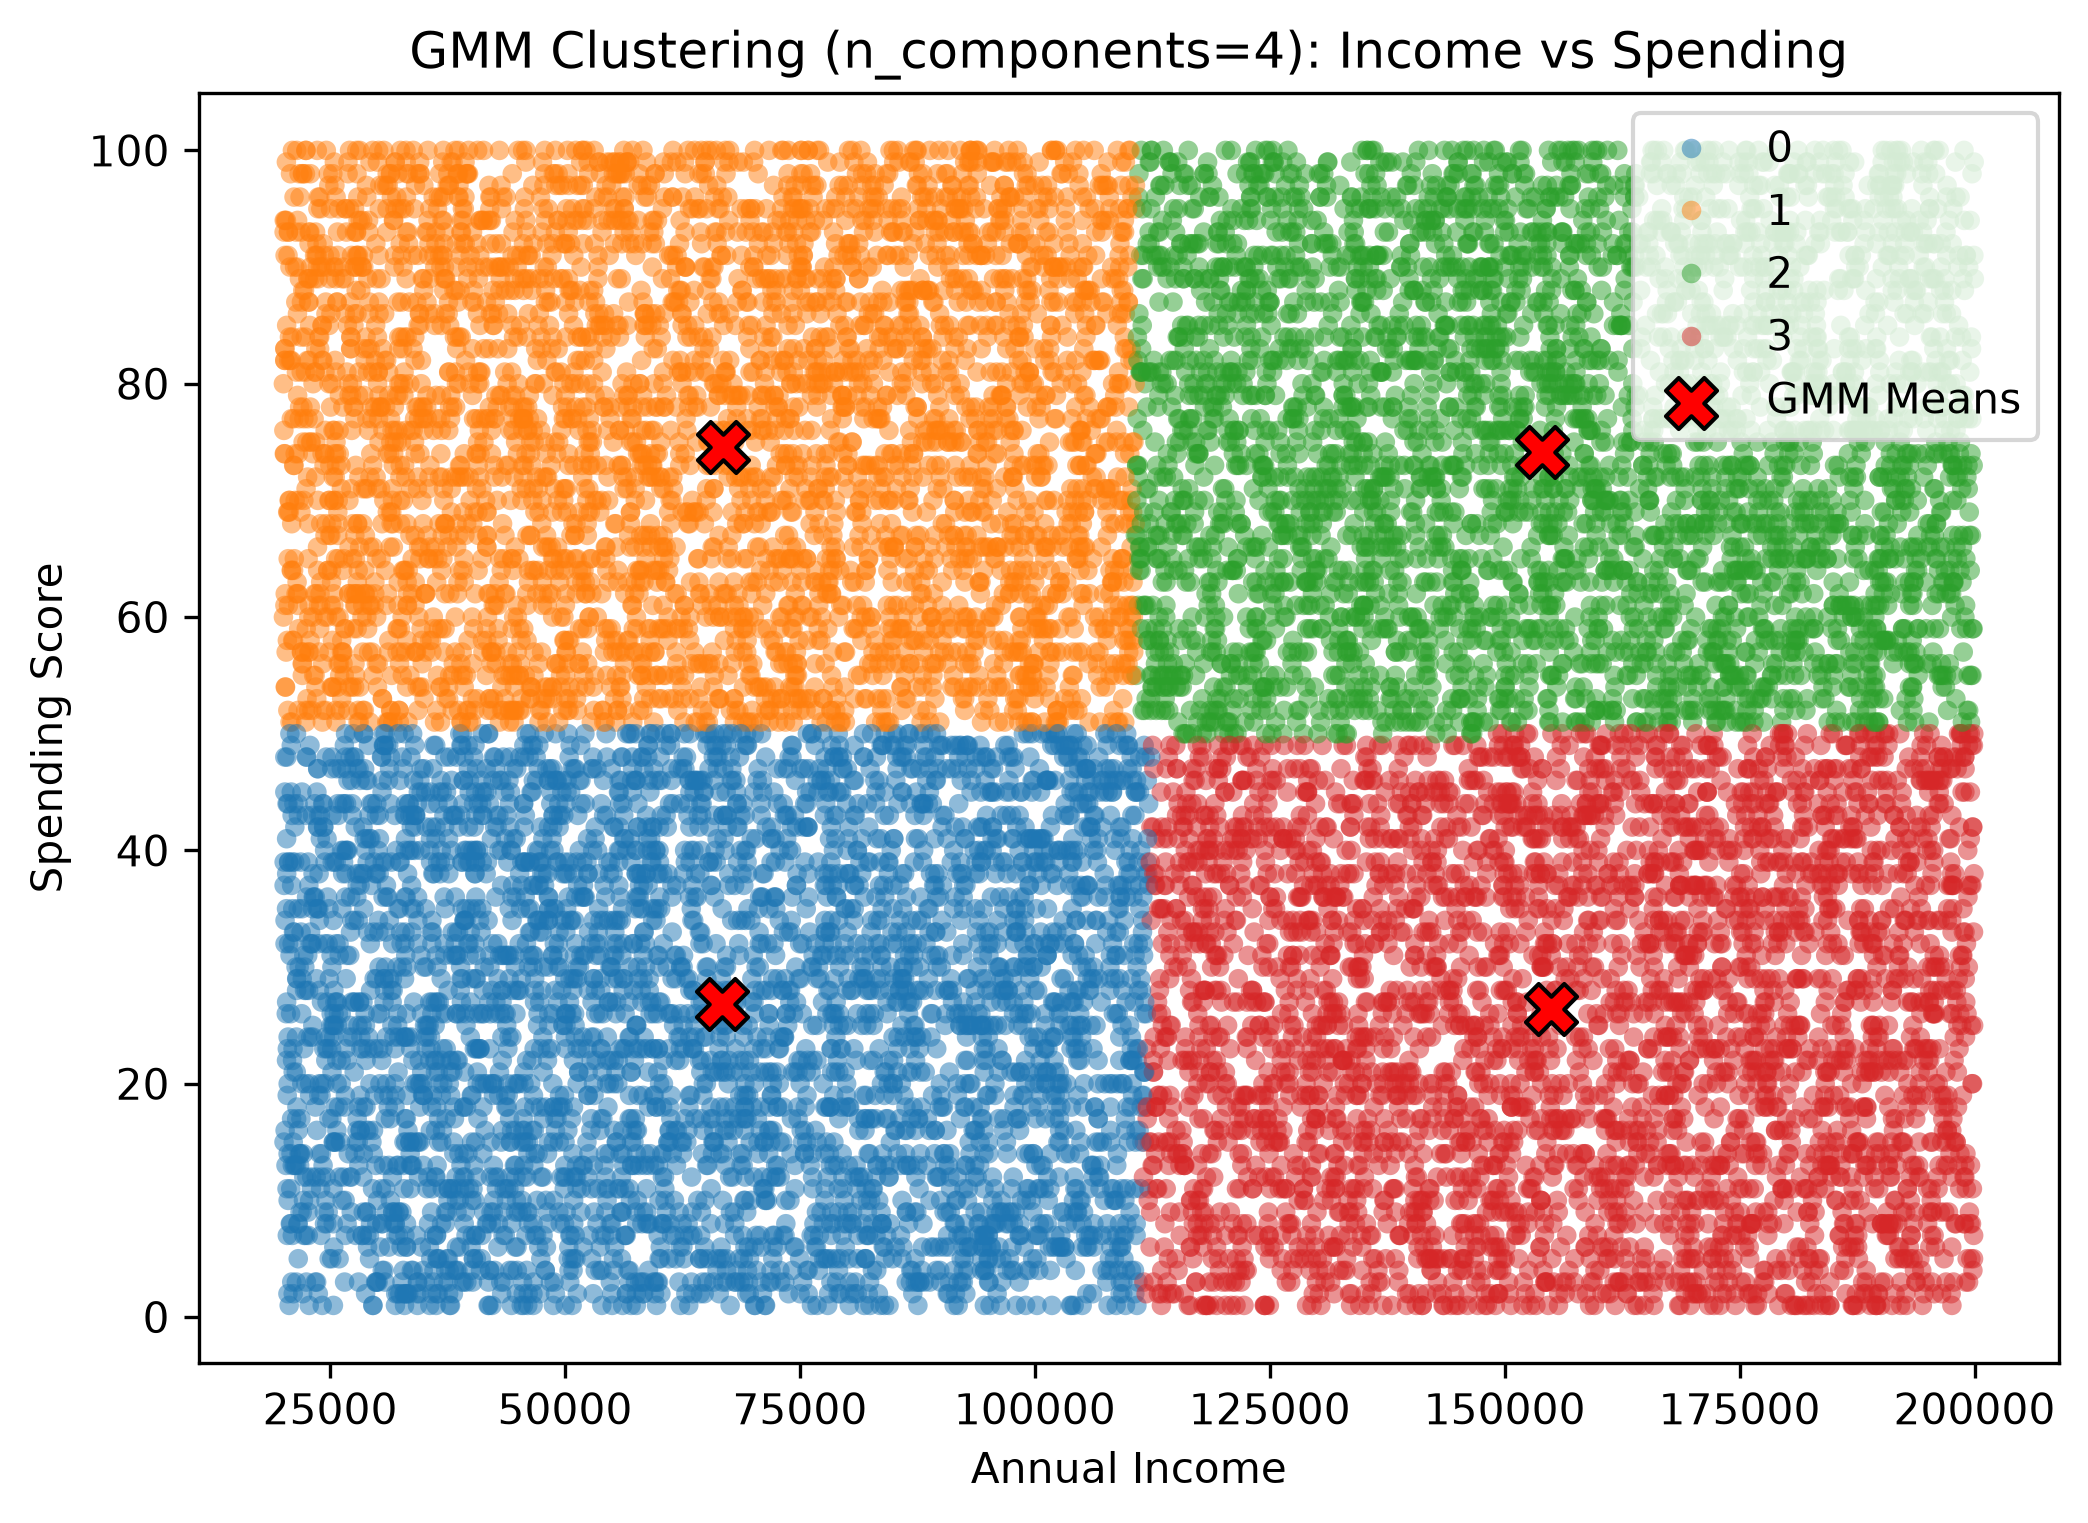
\includegraphics[width=\textwidth]{figures/lab03/gmm_income_vs_spending.png}
  \caption{GMM on Income vs.\ Spending --- soft cluster memberships shown via color blending where points have non-trivial probability of belonging to multiple components.}
\end{figure}

\begin{figure}[H]
  \centering
  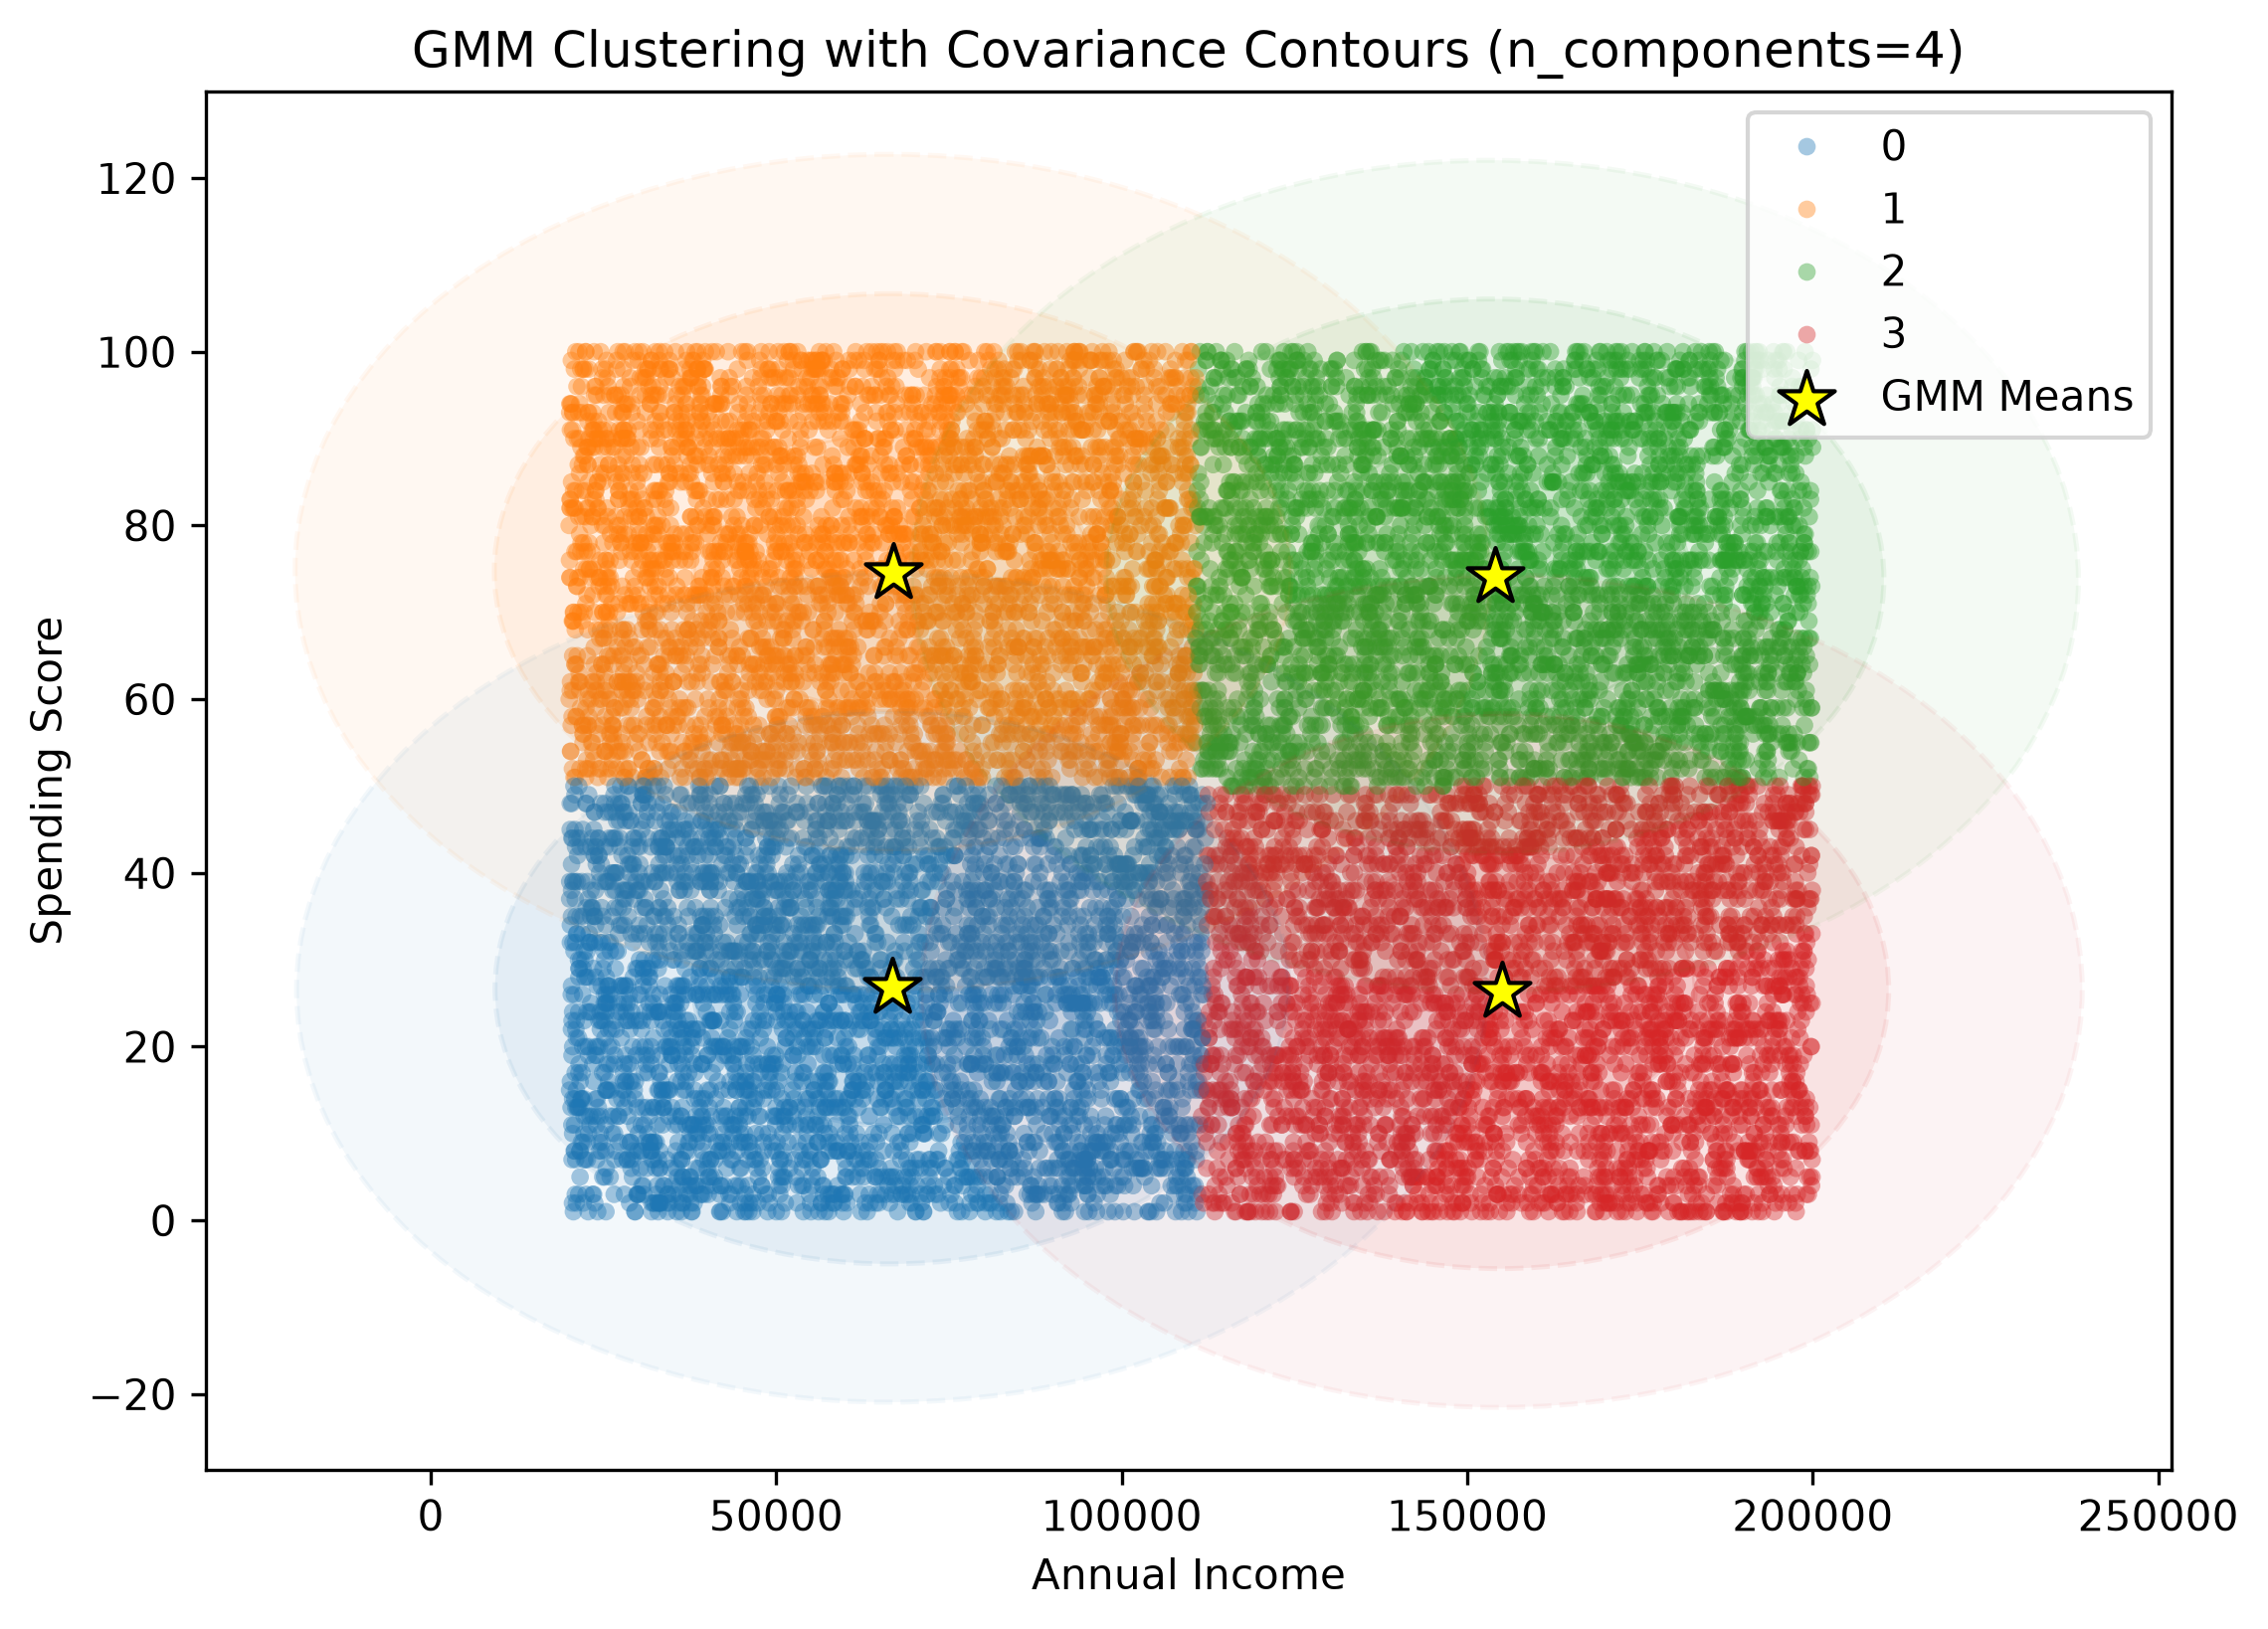
\includegraphics[width=\textwidth]{figures/lab03/gmm_contours.png}
  \caption{GMM covariance contours at $1\sigma$, $2\sigma$, and $3\sigma$ --- ellipses are roughly circular, confirming that cluster covariances are near-isotropic and supporting K-Means's spherical assumption.}
\end{figure}

\subsection{Segment Profiling}

Each cluster's statistical fingerprint is translated into a human-readable name and concrete marketing action. The five clusters partition the 2,200 customers into segments with clear behavioral signatures:

\begin{table}[H]
\centering\rowcolors{2}{tablerow}{white}
\begin{tabular}{c L{3.2cm} c c c L{3.5cm}}
\toprule\rowcolor{tablehead!80}\color{white}\textbf{Cl.} &\color{white}\textbf{Name} &\color{white}\textbf{Size} &\color{white}\textbf{Income} &\color{white}\textbf{Spending} &\color{white}\textbf{Strategy}\\
\midrule
0 & High Inc, Low Spend & 497 & \$91.2k & 16.6 & Incentives to convert\\
1 & Low Inc, Low Spend & 258 & \$26.0k & 22.1 & Low-cost engagement\\
2 & Moderate & 712 & \$53.2k & 47.7 & Retention \& seasonal offers\\
3 & High Inc, High Spend & 242 & \$83.9k & 80.7 & Loyalty \& premium perks\\
4 & Low Inc, High Spend & 491 & \$27.2k & 70.4 & Bundles \& value promos\\
\bottomrule
\end{tabular}
\caption{Five segments with recommended business actions}
\end{table}

Cluster 2 (Moderate) is the largest at 712 customers (32.364\%), forming the ``average'' segment that anchors the mall's baseline revenue. Cluster 3 (High Inc, High Spend) is the smallest at 242 customers (11.000\%) but represents the highest lifetime-value segment: these customers combine high purchasing power with high willingness to spend, making them ideal candidates for loyalty programs and premium product lines. Cluster 0 (High Inc, Low Spend) contains 497 customers (22.591\%) and is the most actionable opportunity --- these customers have the means to spend but currently do not; targeted incentives, personalized offers, and improved in-store experience could convert a meaningful fraction of this segment into high-spending customers. Clusters 1 and 4 share low income but differ sharply in spending behavior: Cluster 4's 491 customers (22.318\%) spend aggressively despite modest means, while Cluster 1's 258 customers (11.727\%) are conservative spenders. The marketing cost per customer must be calibrated to expected return --- high-cost campaigns targeted at Cluster 1 would likely generate negative ROI, whereas even modest promotions to Cluster 4 could yield high conversion rates.

\subsection{Deployment Check}
The fitted estimator, preprocessing transformer, feature names, and metadata are bundled into a single \texttt{joblib} file. A verification check loads the bundle and predicts a cluster for a dummy customer (35F, \$60K income, spending 50) to confirm end-to-end inference works independently of notebook state. The pipeline is self-contained: the exported artifact includes the scaler parameters and centroid coordinates, so the deploying system needs only \texttt{joblib} and \texttt{numpy}, with no dependency on the original training notebook or dataset.

\section{Results and Analysis}

\begin{resultbox}
\textbf{Selected model:} K-Means, \textbf{K=5}, features = \texttt{income\_spending\_only}, \textbf{RobustScaler}.\\
\textbf{Silhouette: 0.470} --- well-separated clusters with strong structure, substantially above the 0.300 success threshold.
\end{resultbox}

\begin{figure}[H]
  \centering
  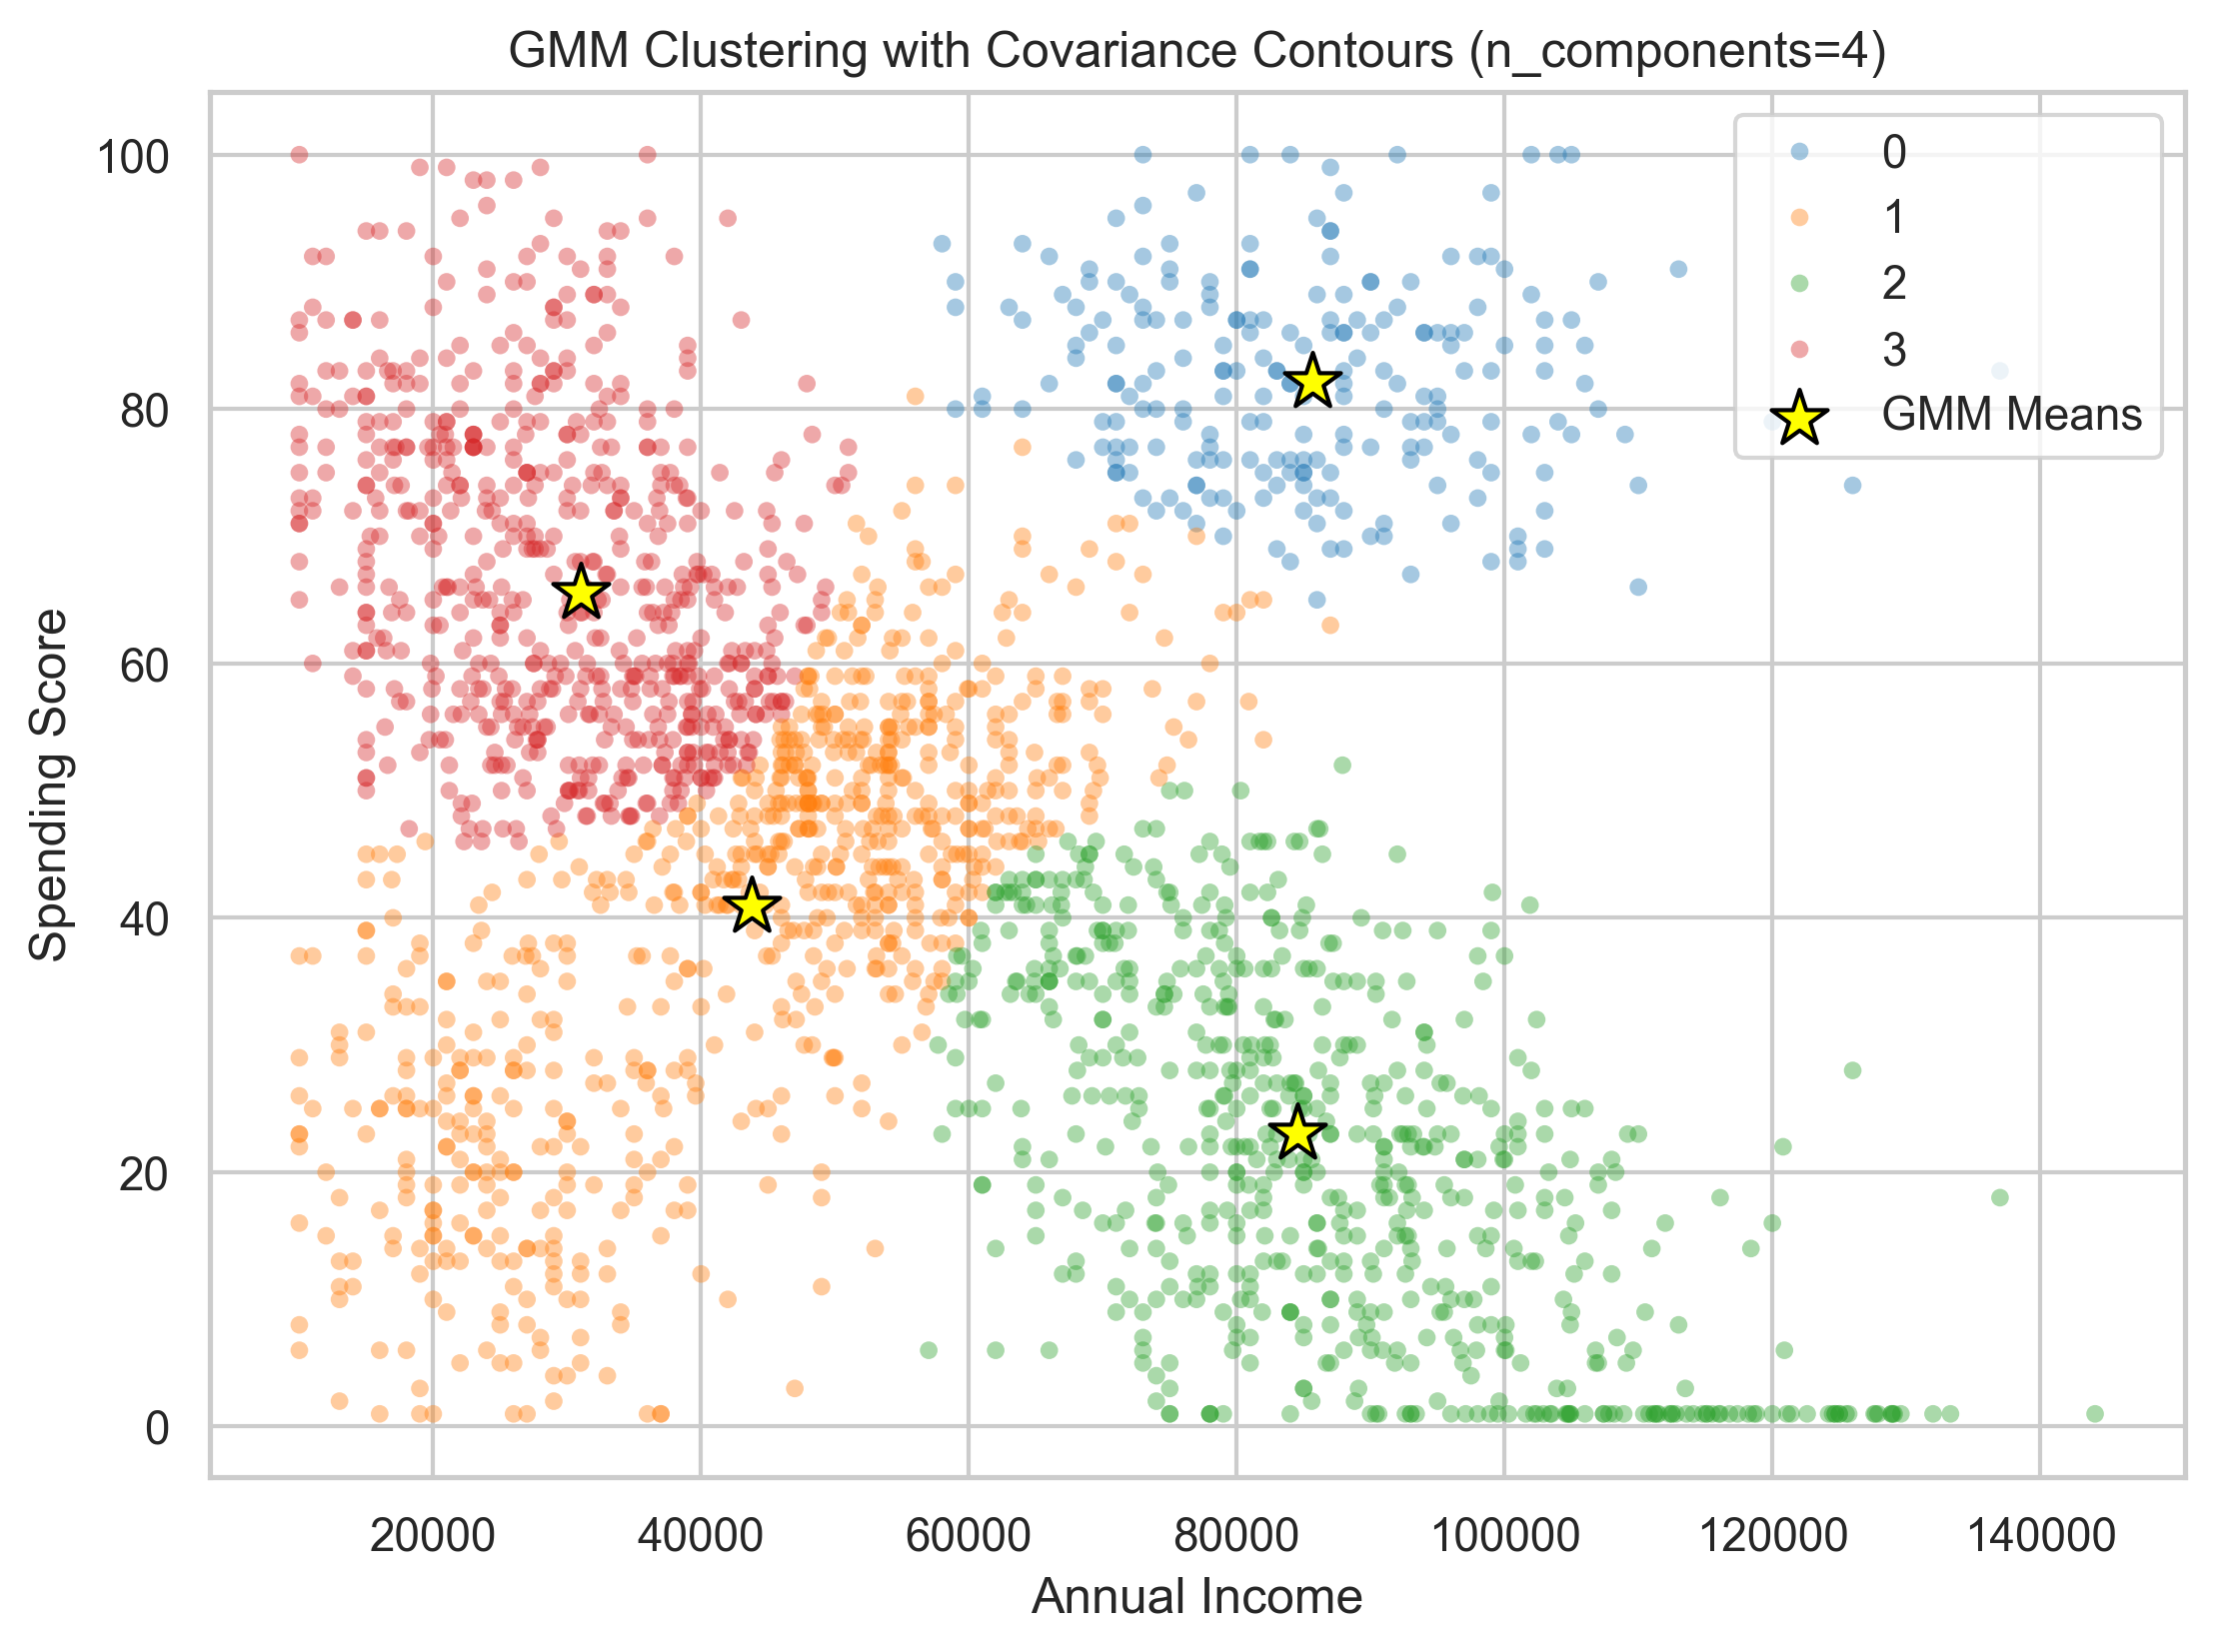
\includegraphics[width=0.700\textwidth]{figures/lab03/gmm_contours_comparison.png}
  \caption{GMM with 4 components and covariance contours on Income vs.\ Spending scatter. Ellipses at $1\sigma$, $2\sigma$, and $3\sigma$ reveal cluster shape and orientation --- most components are near-circular, confirming that the spherical K-Means assumption holds well for these data.}
\end{figure}

\begin{figure}[H]
  \centering
  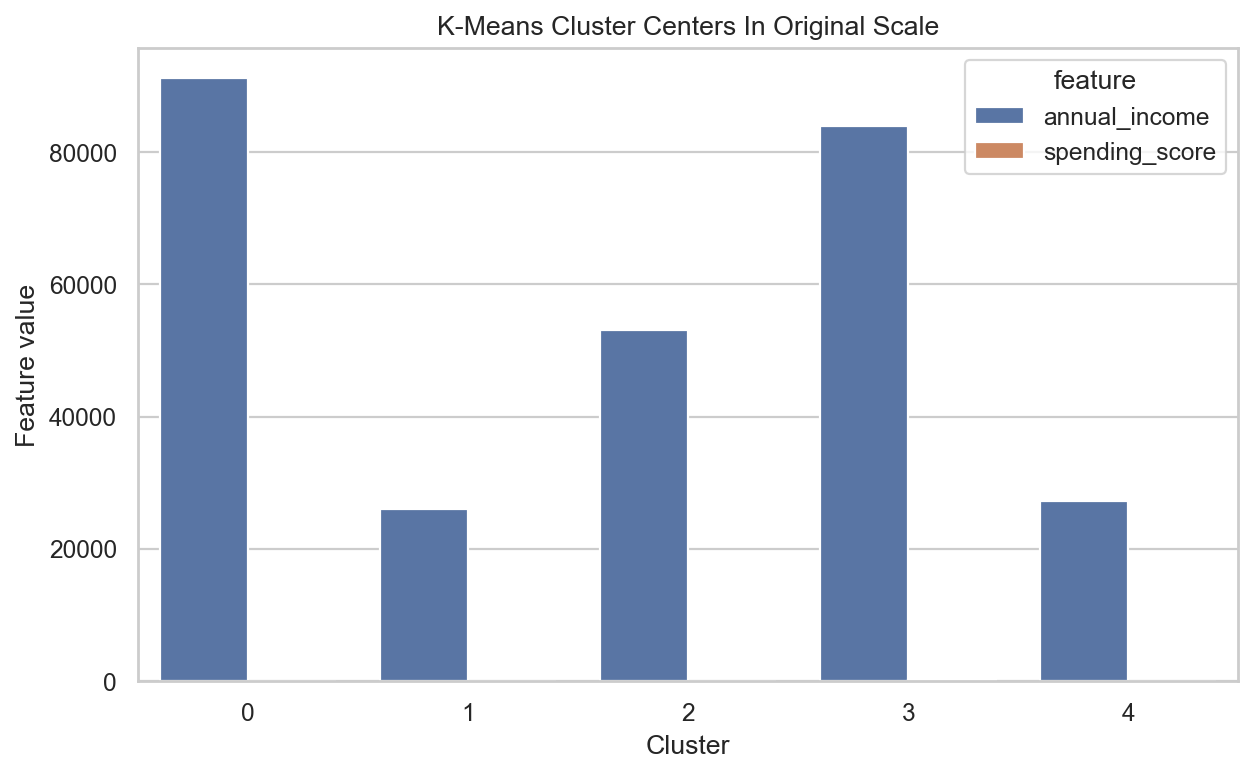
\includegraphics[width=0.780\textwidth]{figures/lab03/cluster_centers_original_scale.png}
  \caption{Cluster centers in original feature scale --- inverse-transformed from StandardScaler for business-interpretable segment profiles. The five centroids map cleanly onto the five behavioral archetypes identified in the segment profiling table.}
\end{figure}

\begin{figure}[H]
  \centering
  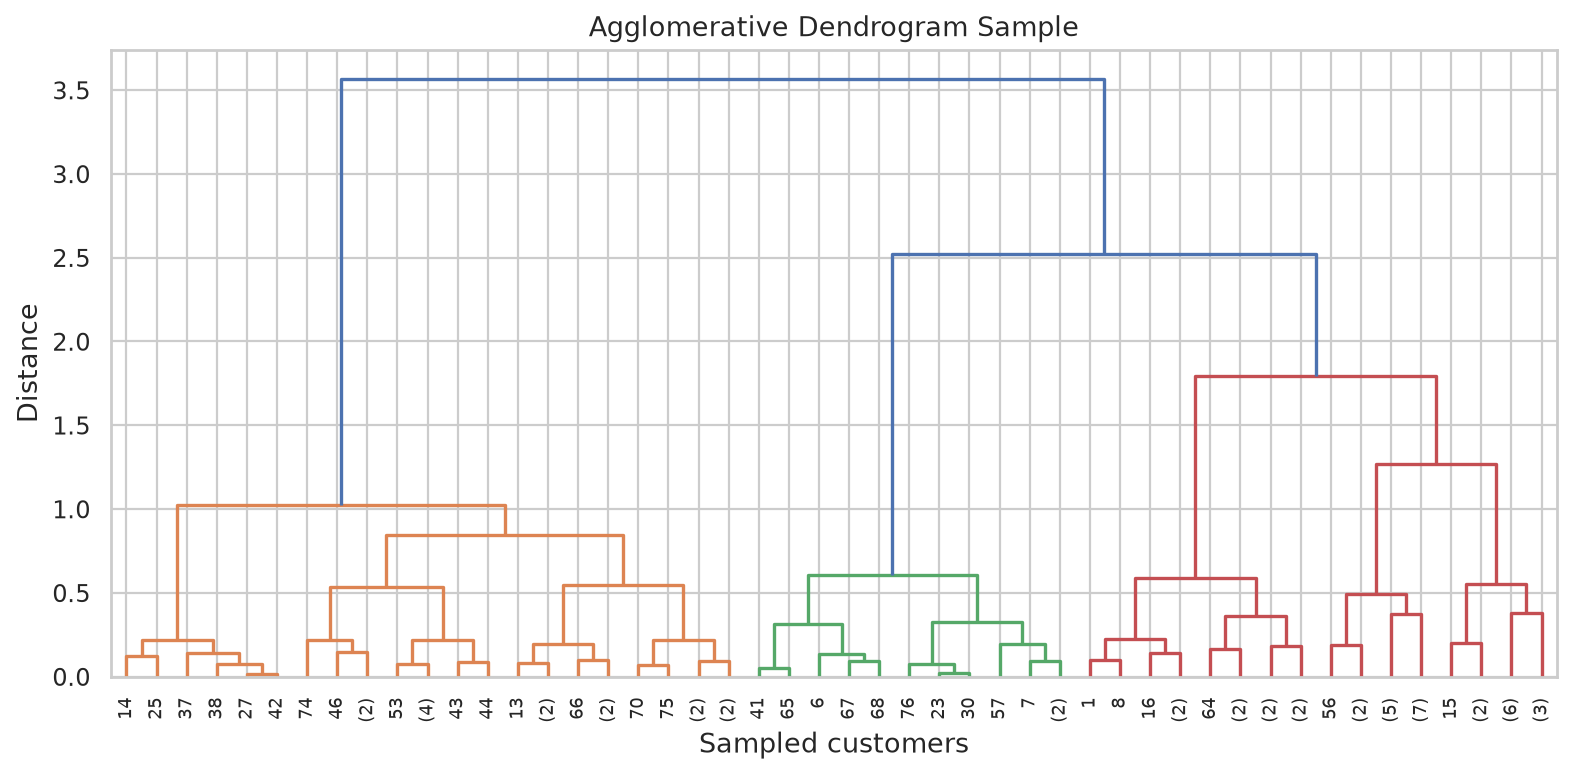
\includegraphics[width=0.780\textwidth]{figures/lab03/agglomerative_dendrogram_sample.png}
  \caption{Agglomerative clustering dendrogram --- hierarchical view of cluster merging distances on a sample subset. The dendrogram confirms that five is a natural cut point: the merge distance increases sharply when reducing from 5 to 4 clusters, indicating that the five-cluster solution captures genuine structure rather than an arbitrary partition.}
\end{figure}

\begin{notebox}
\textbf{Income and Spending together reveal 5 distinct, actionable groups.} Cluster 3 (High Inc, High Spend, 242 customers) is the most valuable segment --- smallest in size but highest in lifetime value per customer. Cluster 1 (Low Inc, Low Spend, 258 customers) requires the lightest engagement touch: high-cost marketing campaigns directed at this segment would produce negative ROI. Cluster 0 (High Inc, Low Spend, 497 customers) presents the largest untapped revenue opportunity --- these customers possess the financial capacity to spend but are not yet doing so. Multi-criteria model selection proves essential in this workflow: optimizing any single metric in isolation would have been misleading. Maximizing silhouette alone could favor an uninterpretable or uneven partition; minimizing inertia blindly would select $K=10$, splitting natural groups into micro-clusters with no business meaning. The combination of statistical quality (silhouette = 0.470), visual coherence (five distinct clouds in the income-spending plane), and business interpretability (each cluster maps to a distinct, nameable behavioral archetype) justifies the final model choice with rigor that no single-number criterion could achieve.
\end{notebox}
